\documentclass[11pt]{article}

\usepackage[margin=1.05in]{geometry}
\usepackage{amsmath,amssymb,amsthm}
\usepackage{mathtools}
\usepackage{graphicx}
\usepackage{booktabs}
\usepackage{array}
\usepackage{microtype}
\usepackage{xcolor}
\usepackage[shortlabels]{enumitem}
\usepackage[colorlinks=true,linkcolor=blue!45!black,citecolor=blue!45!black,urlcolor=blue!45!black]{hyperref}
\hypersetup{pdftitle={The golden-ratio threshold for a lattice Levy walk and ties in coin-turning walks},pdfauthor={Arjun Pemmasani}}

% ---------- theorem environments ----------
\newtheorem{theorem}{Theorem}[section]
\newtheorem{lemma}[theorem]{Lemma}
\newtheorem{proposition}[theorem]{Proposition}
\newtheorem{corollary}[theorem]{Corollary}
\newtheorem{conjecture}[theorem]{Conjecture}
\theoremstyle{definition}
\newtheorem{definition}[theorem]{Definition}
\newtheorem{example}[theorem]{Example}
\theoremstyle{remark}
\newtheorem{remark}[theorem]{Remark}

% ---------- notation macros ----------
\newcommand{\Z}{\mathbb{Z}}
\newcommand{\E}{\mathbb{E}}
\newcommand{\Prob}{\mathbb{P}}
\newcommand{\Var}{\operatorname{Var}}
\newcommand{\CP}{\mathrm{CP}}
\newcommand{\draftloc}[1]{\hyperref[fn:evdraft]{\textup{(author draft, #1)}}}

\title{The golden-ratio threshold for a lattice L\'evy walk\\ and ties in coin-turning walks}
\author{Arjun Pemmasani\\[2pt]
\small Department of Mathematics, Harvey Mudd College\\
\small Claremont, CA 91711, USA\\
\small \texttt{apemmasani@hmc.edu}\\
\small ORCID \href{https://orcid.org/0009-0001-2776-6298}{0009-0001-2776-6298}}
\date{}
\begin{document}
\maketitle

\begin{abstract}
We study the golden-ratio threshold for a lattice L\'evy walk, an alternating
renewal walk on $\Z$ started in equilibrium, with independent run lengths of
tail $k^{-\alpha}$, $1<\alpha<2$. We
compare the probability of each end, $\pm N$, after $N$ steps with that of
the center. Wang, Li and H\"anggi (2016) observed, as a heuristic, that the
ends and the center decay at the same rate when $\alpha$
is the golden ratio. We prove the lattice form of their observation, with its
constant. The ends beat the center for large $N$ exactly when $\alpha$
is below the golden ratio, and at the golden ratio the center still wins by a
constant factor. The proof rests on a local limit theorem at the center, which
holds for every first run that is finite almost surely. For runs of infinite
mean we prove a local form of Lamperti's law at the center. We also study an aging walk (the coin-turning walk), which switches at step
$k$ with probability $c/k$. With a fixed first step, every interior position ties with
the end exactly at $c=1$, for every $N$. The same holds for an aging walk with
$d$ states, whose vector of counts is exactly uniform at the tie.
\end{abstract}

\medskip
\noindent\textbf{Keywords.} L\'evy walk, alternating renewal process, local
limit theorem, persistent random walk, coin-turning walk, P\'olya urn.

\noindent\textbf{Mathematics Subject Classification (2020).} Primary 60G50,
60K05. Secondary 60F05, 60J10, 60C05, 82C41, 82C70.

\section{Introduction}\label{sec:intro}

We study walks on $\Z$ that move in runs of alternating direction with random
lengths. Let $A_N$ be the number of right steps among the first $N$. If the run
lengths are independent, $A_N$ is the occupation time of an alternating
renewal process~\cite{godrecheluck2001,lamperti1958}. If they are also
heavy-tailed, the walk is a lattice analogue of a L\'evy walk. L\'evy walks
are a standard model of superdiffusion~\cite{zdk2015}, and they also describe
anomalous heat transport in one-dimensional lattices~\cite{dsd2013,wlh2016}.
The profile of a L\'evy walk has a central peak and two ballistic side
peaks~\cite{zdh2011,dzh2012,zdk2015}, and the part of the profile between
them is described by an infinite density~\cite{rdhb2014,rdhb2014b}.

On the lattice we compare the end bins $A_N=N$
and $A_N=0$, which the walk reaches only if one run covers all $N$ steps, with
the center $A_N=N/2$, which it reaches in many ways. In the picture of heat
spreading, the end bins are the lattice form of the ballistic side peaks of
the standard L\'evy walk (the walk without velocity fluctuations, see
Remark~\ref{rem:humps}). The
center bin is the top of the central peak, and the stationary start used below
is the equilibrated initial ensemble~\cite{dzh2012}. We ask when the ballistic
ends beat the center.

For runs with geometric lengths this question is
Problem~131 of Kagey's Open Problem Collection~\cite{kagey131}, posed for a
Galton board. The walk is then the persistent random
walk~\cite{kac1974,renshawhenderson1981}, which remembers
only its last step, and the center catches up with the ends when the expected
number of switches is about $\log N$~\cite{paperA}.

In this paper we ask what happens if the walk remembers more. We study two
kinds of memory.
\begin{itemize}[nosep]
\item A walk with heavy-tailed runs remembers how long it has gone in its
current direction. Its path is a sequence of runs of alternating direction,
and the run lengths $\xi$ are independent with $\Prob(\xi\ge k)=k^{-\alpha}$
for $k\ge1$.
\item An aging walk remembers how old it is. It switches at step $k\ge2$ with
probability $c/k$. This is the coin-turning walk of Engl\"ander and
Volkov~\cite{ev2018,evw2020} with $p_k=c/k$. (In the literature on renewal processes and L\'evy
walks, aging means instead that the process depends on the time since it was
prepared~\cite[Sections~8 and~9]{godrecheluck2001}.) We also give the walk $d$ directions. Then at step $k\ge2$
it turns to each of the other $d-1$ directions with probability
$\theta/(k+d-2)$, which is $c/k$ with $c=\theta$ when $d=2$.
\end{itemize}

\subsection{Why the golden ratio}\label{sec:heuristic}

Here is the heuristic. Theorem~\ref{thm:center} and Corollary~\ref{cor:golden} make it rigorous.
For heavy-tailed runs take $1<\alpha<2$, so a run has a finite mean $\mu$ but
an infinite variance. Start the walk in equilibrium, at a typical time of a
long sequence of runs. Then the first run is already in progress, and long runs
are more likely to be in progress. The chance that this run covers all $N$
steps is of order $N^{1-\alpha}$, and this is the order of the end. For the center, the runs
to the right and the runs to the left form two independent renewal processes,
each making about $N/(2\mu)$ runs, and the walk ends in the center when they
meet at level $N/2$. Each process fluctuates on the scale $N^{1/\alpha}$ of a
stable law, so they meet at the same level with probability of order
$N^{-1/\alpha}$. Hence the ratio of end to center is
of order $N^{1-\alpha}/N^{-1/\alpha}=N^{1-\alpha+1/\alpha}$. The exponent
vanishes when $\alpha^2-\alpha-1=0$, that is, at the golden ratio
$\alpha=\varphi=(1+\sqrt5)/2$. Below
$\varphi$ the ends win, and above $\varphi$ the center wins. If the first run
is a fresh run instead, the end is of order $N^{-\alpha}$, a factor $N$
smaller, and the center wins for every $1<\alpha<2$.

\subsection{Setting and notation}\label{sec:notation}

Every walk in this paper takes $N$ steps $X_1,\dots,X_N\in\{+1,-1\}$, where
$+1$ means right. Let $A_N=\#\{i\le N:X_i=+1\}$ be the number of right steps,
and write $P_N(k)=\Prob(A_N=k)$ for the probability of bin $k$, that is, of
$k$ right steps, for whichever walk we study. Unless we say otherwise the first
step is fair, $\Prob(X_1=+1)=\frac12$, and the rules treat the two directions
alike, so $P_N(k)=P_N(N-k)$. We write $\Prob_+$ and $\E_+$ for probability and
expectation given $X_1=+1$. For even $N$ we put $h=N/2$ and call
$C_N=P_N(h)$ the center and $E_N=P_N(N)=P_N(0)$ the end. Whenever $C_N$
appears, $N$ is even. A crossing is a value of the parameter at which a bin
ties with an end, and for the center this means $C_N=E_N$. For
heavy-tailed runs we do not locate a crossing at fixed $N$. There we prove
which of $C_N$ and $E_N$ is larger for all large $N$ at fixed $\alpha$, and
the golden ratio is the threshold for this sign.

All logarithms are natural,
$H_k=\sum_{j\le k}1/j$ is the $k$-th harmonic number, and $\gamma$ is Euler's
constant. Limits, $O(\cdot)$ and $o(\cdot)$ refer to $N\to\infty$, over even
$N$ when $C_N$ appears. The constants implied by $O(\cdot)$ are absolute
unless we name what they depend on.

Heavy-tailed runs (Section~\ref{sec:heavy}) have
the exponent $\alpha$, the mean run length $\mu=\E\xi=\zeta(\alpha)$ for
$\alpha>1$, and the length $D$ of the first run. A fresh start has $D$
distributed as $\xi$, and the stationary start has
$\Prob(D=\ell)=\Prob(\xi\ge \ell)/\mu$. We put $R_N=E_N/C_N$, so the ends win
exactly when $R_N>1$. The aging walk (Section~\ref{sec:aging}) has the
constant $c\in(0,2)$, and its version with $d$ states has the constant
$\theta$ and the count vector $(n_1,\dots,n_d)$, where $n_i$ is the number of
steps in state $i$. Symbols that only one section uses are defined in that
section.

\subsection{Results}\label{sec:results}

In both models the start matters. For heavy-tailed runs it decides whether
the threshold is $\varphi$ or $1$, and for the aging walk it decides whether
the crossing is exactly $c=1$. The main results are Theorem~\ref{thm:center}
and Corollary~\ref{cor:golden} for heavy-tailed runs and
Proposition~\ref{prop:aging-two} and Theorem~\ref{thm:aging-d} for aging
walks. Theorems~\ref{thm:center}, \ref{thm:alpha2} and~\ref{thm:lamperti} are
proved in Appendix~\ref{app:heavy}, and
Proposition~\ref{prop:aging-expansion} in Appendix~\ref{app:aging}. The other
results are proved where they are stated.

\paragraph{Heavy-tailed runs.}
For $1<\alpha<2$ and every first run that is finite almost surely, $C_N$ is
asymptotic to an explicit constant times $N^{-1/\alpha}$
(Theorem~\ref{thm:center}). With the stationary start
$R_N\sim C(\alpha)N^{1-\alpha+1/\alpha}$ for an explicit constant $C(\alpha)$. Here
$C(\varphi)=0.7761\ldots$ (and $C(\varphi)<0.952$ by elementary bounds), so
at $\alpha=\varphi$ the center still wins. With a fresh start $R_N\to0$
(Corollary~\ref{cor:golden}).

For $\alpha\ge2$ the center is of order
$N^{-1/2}$, with an extra factor $(\log N)^{-1/2}$ at $\alpha=2$, and
$R_N\to0$ with either start (Theorem~\ref{thm:alpha2}). For $0<\alpha<1$ the
runs have infinite mean and only the fresh start makes sense. Then
$NC_N\to\frac2\pi\tan\frac{\pi\alpha}2$ and $R_N\to\infty$
(Theorem~\ref{thm:lamperti}). So with a fresh start the ends win for
$\alpha<1$ and the center wins for $\alpha>1$. We do not prove what happens
at $\alpha=1$ (Remark~\ref{rem:other}).

\paragraph{Aging.}
With a fixed first step and $c=1$ the number of right steps is exactly
uniform on $\{1,\dots,N\}$. The ratio of each interior bin to the end
increases strictly in $c$, so every interior bin ties with the end exactly at
$c=1$, for every $N\ge2$ (Proposition~\ref{prop:aging-two}). With $d$ states,
a start in state~$1$ and $\theta=1$, the count vector is exactly uniform over
all compositions $(n_1,\dots,n_d)$ of $N$ with $n_1\ge1$, and every other
such bin ties with the corner $(N,0,\dots,0)$ exactly at $\theta=1$, for
every $N\ge2$ (Theorem~\ref{thm:aging-d}). A small change of the aging rate
gives a chain that redraws or repeats its state, and its counts have exactly
the law of P\'olya's urn for every weight
(Proposition~\ref{prop:aging-urn}).

With a fair first step each
interior bin is twice as likely as an end at $c=1$, and its crossing is
unique and below $1$ (Proposition~\ref{prop:aging-fair}). For the center the
crossing is
$c_N=1-\log2/(\log N+\gamma+2-2\log2)+O((\log N)^{-3})$
(Proposition~\ref{prop:aging-expansion}).

\paragraph{Methods.}
For heavy-tailed runs the walk is made of two independent renewal processes,
one for the runs of each sign (Proposition~\ref{prop:tworenewal}). At the
center we need a local limit theorem for each of them, with a delay for the
first run. We obtain it from Gnedenko's local limit theorem for the sums of the
run lengths. Sums of few runs that lie far above their mean are controlled by
local bounds in the big-jump domain. For $\alpha<1$ these bounds need one more
step, in which we cut the runs into two halves. Then a Mellin transform
identifies the limit with Lamperti's density.

For the aging walk all the exact
laws come from one chain that draws afresh or repeats its state. The ties come
from writing each ratio of a bin to the end as a sum over paths of products of
odds that increase in $c$. For the fair start we couple the walk with the
chain that draws afresh or repeats, whose counts are a mixture of binomial
laws, and summation by parts turns the coupling into a local limit theorem
with a rate.

\subsection{Prior work}\label{sec:prior}

For heavy-tailed runs, Godr\`eche and Luck~\cite{godrecheluck2001} give the
transform of the occupation time of an alternating renewal process started at
a renewal. They give the decay of the end for both
starts~\cite[Eqs.~(1.6) and~(8.7)]{godrecheluck2001}, and from the transform
they derive, by a formal Laplace analysis in continuous time, the stable law
of the occupation time for
$1<\alpha<2$~\cite[Section~7(iii), Eqs.~(7.12) to~(7.15)]{godrecheluck2001}. Read at the center, that
law gives the constant of Theorem~\ref{thm:center}.

In probability theory the
walk is the one-dimensional directionally reinforced random walk of Mauldin,
Monticino and von Weizs\"acker~\cite{mmw1996}, whose limit laws were found by
Horv\'ath and Shao~\cite{horvathshao1998}. C\'enac, Le~Ny, de~Loynes and Offret
study it as a persistent random walk whose runs have general lengths. They give
criteria for recurrence~\cite{clnlo2018} and prove functional scaling
limits~\cite{clnlo2019}, namely a Brownian motion for $\alpha\ge2$, a stable L\'evy
process for $1<\alpha<2$~\cite[Theorem~3.2]{clnlo2019} and an arcsine Lamperti
process for $\alpha<1$~\cite[Theorem~3.3 and Eq.~(3.25)]{clnlo2019}. Theorems~\ref{thm:center},
\ref{thm:alpha2} and~\ref{thm:lamperti} are local forms of the marginals of
these limits at the center. The end $E_N$ is a persistence event, and it is
not a local form of these limits. Magdziarz, Scheffler, Straka and
\.Zebrowski~\cite{mssz2015} prove limit theorems for L\'evy walks in continuous
space and time.

The scalings of the central peak and of the side
peaks were known before~\cite{cdp2005,zdh2011,dzh2012,zdk2015}, but we did
not find the balance of the two stated there. The observation that equal
decay of the two singles out the golden ratio is due, as far as we know, to
Wang, Li and H\"anggi~\cite[Section~6.2.1.3, Eq.~(6.49)]{wlh2016}, who used it as a
heuristic for the exponent of anomalous heat conduction. They also mention that
Lee-Dadswell, Nickel and Gray~\cite{ldng2005} had found the same conduction
exponent $(3-\sqrt5)/2$ by a hydrodynamic argument. The two decay rates of the end,
$N^{1-\alpha}$ and $N^{-\alpha}$, are the scalings of the ballistic peaks of a
L\'evy walk with and without an equilibrated start~\cite[Table~I]{dzh2012}.

What we add for heavy-tailed runs is a lattice local limit theorem at the
center for every first run that is finite almost surely, so for both starts.
With it the comparison of the end with the center becomes a theorem with the
explicit constant $C(\alpha)$, and at $\alpha=\varphi$ the center wins
strictly. For $\alpha<1$ the limit law of $A_N/N$ is
Lamperti's~\cite{lamperti1958}, and we prove its local form at the center. We
found only the integral law in the literature.

For aging walks, Dietz and Sethuraman~\cite{ds2007} proved the limit law of
$A_N/N$, Engl\"ander and Volkov~\cite{ev2018} gave a second proof, and
Engl\"ander, Volkov and Wang~\cite{evw2020} found the scaling limit of the
walk. For $d$ states the limit is a Dirichlet
law~\cite[Theorem~1.4]{ds2007}, and Bouguet and
Cloez~\cite[Propositions~4.1 and~4.5]{bc2018} find the joint limit of the
fractions of time and the current state. The exact uniform law for two states is an
exercise in~\cite[Section~3.1, footnote~1]{evw2020}, which also announces a general
connection with P\'olya urns. The law of the counts of the chain of
Proposition~\ref{prop:aging-urn} also follows from a result of Dietz, Lippitt
and Sethuraman~\cite[Theorem~2.18]{dls2023} (Section~\ref{sec:aging-urn}).

Chapter~7 of the March 18, 2024 author draft of Engl\"ander and
Volkov's monograph~\cite{ev2025} gives the two-state joint law with the last
state, including the uniform case and positive integer urn weights.\footnote{\label{fn:evdraft}
The dated author upload is at
\url{https://www.researchgate.net/publication/379333206_Coin-Turning_Random_Walks_and_Inhomogeneous_Markov_Chains}.
All draft locators below refer to this version. We have not checked the
numbering of the published edition.}
Section~\ref{sec:aging} gives the precise overlaps and the time shift,
separating the count law from the joint law and from the path law.

Pradhan, Roy and Ray~\cite{prr2026} study, with the methods of physics, a
persistent walk whose probability of reversal decays like a power of the time.
When the power is one it is close to our aging walk, and they find its second
moment and the tail of its runs.

What we add in
Section~\ref{sec:aging} is the joint law of the counts and the last state for
$d\ge3$ states or a weight $\theta$ that is not an integer,
the strict ordering that turns the uniform laws into ties
(Proposition~\ref{prop:aging-two}(b) and Theorem~\ref{thm:aging-d}(b)), and
for the fair start the expansion of the crossing
(Proposition~\ref{prop:aging-expansion}) with the local limit theorem with a
rate behind it (Proposition~\ref{prop:D-llt}).

\section{Heavy-tailed runs}\label{sec:heavy}

In this section the walk remembers the time since its last switch, and we
compare its ends with its center for every exponent $\alpha>0$. The steps
form maximal runs whose directions alternate. The first run has length $D$,
and the later runs have i.i.d.\ lengths $\xi_1,\xi_2,\dots$ distributed as
$\xi$, where
\[
 \bar F(k)=\Prob(\xi\ge k)=k^{-\alpha}\quad(k\ge1)
\]
for some $\alpha>0$. So $\Prob(\xi=k)=k^{-\alpha}-(k+1)^{-\alpha}>0$ for every
$k\ge1$. The first direction is fair, and $D$, $(\xi_i)$ and the first
direction are independent.

With a fresh start $D$ has the law of $\xi$. For
$\alpha>1$ the stationary start is $\Prob(D=\ell)=\bar F(\ell)/\mu$, where
$\mu=\E\xi=\zeta(\alpha)$. This law is stationary in the following sense. The
number of steps left in the current run, counting the current one, is a Markov
chain that moves from $k\ge2$ to $k-1$ and from $1$ to a fresh copy of $\xi$.
Since $\bar F(k)=\bar F(k+1)+\Prob(\xi=k)\bar F(1)$, the law $\bar F(k)/\mu$
is invariant for this chain. So the stationary start sees the runs at a
typical time. We define $A_N$, $P_N$, $C_N$, $E_N$ and $R_N=E_N/C_N$ as in
Section~\ref{sec:notation}. In this section the constants implied by
$O(\cdot)$ may depend on $\alpha$.

\begin{proposition}[the end]\label{prop:edge}
For every law of $D$ and every $N\ge1$, $E_N=\frac12\Prob(D\ge N)$. With a fresh start
$E_N=\frac12N^{-\alpha}$. With the stationary start
\[
 E_N=\frac{\zeta(\alpha,N)}{2\zeta(\alpha)}
 =\frac{N^{1-\alpha}}{2(\alpha-1)\zeta(\alpha)}\Bigl(1+\frac{\vartheta_N(\alpha-1)}N\Bigr)
\]
for some $\vartheta_N\in[0,1]$, where $\zeta(\alpha,N)=\sum_{k\ge N}k^{-\alpha}$
is the Hurwitz zeta function.
\end{proposition}

\begin{proof}
All $N$ steps are $+1$ exactly when the first direction is $+$ and $D\ge N$.
Hence $E_N=\frac12\Prob(D\ge N)$. For the fresh start
$\Prob(D\ge N)=\bar F(N)=N^{-\alpha}$. For the stationary start
$\Prob(D\ge N)=\sum_{\ell\ge N}\ell^{-\alpha}/\mu=\zeta(\alpha,N)/\zeta(\alpha)$.
To estimate $\zeta(\alpha,N)$ we compare the sum with an integral. Since
$t^{-\alpha}$ is decreasing,
\[
 \int_N^\infty t^{-\alpha}\,dt\le\zeta(\alpha,N)\le N^{-\alpha}+\int_N^\infty
 t^{-\alpha}\,dt .
\]
The integral equals $N^{1-\alpha}/(\alpha-1)$, and $N^{-\alpha}$ is
$(\alpha-1)/N$ times the integral. This gives the second form.
\end{proof}

So the end only sees the first run, while the center depends on all the runs.
For the center we need the renewal quantities
\begin{gather*}
 \tau_m=\xi_1+\dots+\xi_m,\quad\tau_0=0,\qquad u_m(k)=\Prob(\tau_m=k),\\
 q_m(k)=\Prob(\tau_{m-1}<k\le\tau_m)=\sum_{j\ge1}\bar F(j)u_{m-1}(k-j)
\end{gather*}
for $m,k\ge1$. So $u_m(k)$ is the chance that the $m$-th run ends at level $k$,
and $q_m(k)$ the chance that the $m$-th run covers level $k$. For the delayed
versions let $D$ be independent of $(\xi_i)$, and put
$u^D_m(k)=\Prob(D+\tau_{m-1}=k)$, $q^D_1(k)=\Prob(D\ge k)$ and
$q^D_m(k)=\Prob(D+\tau_{m-2}<k\le D+\tau_{m-1})$ for $m\ge2$. For the
stationary start
$u^D_m(k)=\sum_\ell\frac{\bar F(\ell)}{\mu}u_{m-1}(k-\ell)=q_m(k)/\mu$.

The $+$ runs and the $-$ runs form two independent renewal processes. For
$1\le a\le N-1$ the walk is in bin $a$ at time $N$ exactly when one process
has a run that ends exactly at its level ($a$ for the $+$ runs and $N-a$ for
the $-$ runs) and the other process has a run that covers its level.

\begin{proposition}[two renewal processes]\label{prop:tworenewal}
Let $D$ have any law on $\{1,2,\dots\}$. For $a+b=N$ with $a,b\ge1$,
\[
 \Prob_+(A_N=a)=\sum_{m\ge1}\Bigl[u_m(b)\,q^D_{m+1}(a)+u^D_m(a)\,q_m(b)\Bigr],
\]
and $\Prob_+(A_N=N)=\Prob(D\ge N)$. So for even $N$ and $h=N/2$,
$C_N=\sum_{m\ge1}[u_m(h)q^D_{m+1}(h)+u^D_m(h)q_m(h)]$. For the fresh start
this is $C_N=\sum_mu_m(h)[q_m(h)+q_{m+1}(h)]$.
\end{proposition}

\begin{proof}
We split according to the run that contains step $N$. Let the $+$ runs have
lengths $D,\xi^+_2,\xi^+_3,\dots$ and the $-$ runs
$\xi^-_1,\xi^-_2,\dots$, and let $s^\pm_j$ be the sum of the first $j$ lengths
of each sign, with $s^\pm_0=0$. So $s^+_j$ has law $u^D_j$ and $s^-_j$ has law
$u_j$, and the two sequences are independent. The runs alternate and the
first one is a $+$ run. So the $j$-th $+$ run comes after $j-1$ runs of each
sign and covers the steps in $(s^+_{j-1}+s^-_{j-1},\,s^+_j+s^-_{j-1}]$, and
the $j$-th $-$ run covers $(s^+_j+s^-_{j-1},\,s^+_j+s^-_j]$. Let $N=a+b$.
There are three cases.

Suppose step $N$ is in the first run. Then $A_N=N$, and this happens exactly
when $D\ge N$.

Suppose step $N$ is in the $j$-th $+$ run with $j\ge2$. Then exactly $j-1$ of
the $-$ runs lie before step $N$, and they are complete, so
$A_N=N-s^-_{j-1}$. So $A_N=a$ means $s^-_{j-1}=b$, and then step $N=a+b$ is
in this run exactly when $s^+_{j-1}<a\le s^+_j$. By independence this has
probability $u_{j-1}(b)\,q^D_j(a)$.

Suppose step $N$ is in the $j$-th $-$ run. Then the first $j$ of the $+$ runs
are complete and no other has begun, so $A_N=s^+_j$. So $A_N=a$ means
$s^+_j=a$, and then step $N$ is in this run exactly when
$s^-_{j-1}<b\le s^-_j$. This has probability $u^D_j(a)\,q_j(b)$.

The cases are disjoint. Summing them, with $m=j-1$ in the second and $m=j$ in
the third, gives the formula. Now let $N$ be even. The first direction is
fair, and changing the sign of every step sends $A_N$ to $N-A_N$. Hence
$C_N=\frac12[\Prob_+(A_N=h)+\Prob_+(A_N=N-h)]=\Prob_+(A_N=h)$. With a fresh
start $u^D_m=u_m$ and $q^D_m=q_m$, which gives the last formula.
\end{proof}

For a fresh start this identity is the coefficient form of the double transform of Godr\`eche
and Luck~\cite[Section~7]{godrecheluck2001} for the occupation time of an
alternating renewal process. A general first run only changes the factors
$u^D_m$ and $q^D_{m+1}$. To evaluate the sum we need the stable limit of
$\tau_m$ and its local form.

\begin{lemma}[stable and local limits]\label{lem:stable}
Let $1<\alpha<2$ and $a_m=m^{1/\alpha}$. Put
$K_\alpha=\Gamma(2-\alpha)/(\alpha-1)=-\Gamma(1-\alpha)>0$ and
$\sigma_\alpha=2K_\alpha\lvert\cos\frac{\pi\alpha}2\rvert$.
\begin{enumerate}[(i)]
\item $\E e^{i\theta\xi}=1+i\mu\theta+K_\alpha(-i\theta)^\alpha+O(\theta^2)$
as $\theta\to0$, with the principal branch.
\item $(\tau_m-m\mu)/a_m$ converges in law to a variable $G$ with
$\E e^{i\theta G}=\exp(K_\alpha(-i\theta)^\alpha)$. The law of $G$ has a
bounded, uniformly continuous density $g$ with $g(z)\to0$ as
$\lvert z\rvert\to\infty$.
\item (Gnedenko) The constant $\bar u:=\sup_{m\ge1}\sup_ka_mu_m(k)$ is
finite, and $a_mu_m(k)-g((k-m\mu)/a_m)\to0$ uniformly in $k$ as
$m\to\infty$.
\item If $G'$ is an independent copy of $G$, then $G-G'$ is symmetric
$\alpha$-stable with $\E e^{i\theta(G-G')}=e^{-\sigma_\alpha\lvert
\theta\rvert^\alpha}$, and
$I_\alpha:=\int_{\mathbb R}g(z)^2\,dz=\Gamma(1+1/\alpha)/(\pi\sigma_\alpha^{1/\alpha})$.
\end{enumerate}
\end{lemma}

\begin{proof}
All four parts come from the expansion of the transform of $\xi$ near $0$. We
find it first.

(i) Summation by parts gives $1-\E w^\xi=(1-w)\sum_{k\ge1}\bar F(k)w^{k-1}$
for $\lvert w\rvert\le1$. Put $w=e^{-v}$ with $\operatorname{Re}v\ge0$, and
write $\mathrm{Li}_\alpha(w)=\sum_{k\ge1}k^{-\alpha}w^k$. Since
$\bar F(k)=k^{-\alpha}$, the identity reads
$1-\E e^{-v\xi}=(e^v-1)\mathrm{Li}_\alpha(e^{-v})$. For
$0<\lvert v\rvert<2\pi$, \cite[25.12.12]{dlmf} gives
$\mathrm{Li}_\alpha(e^{-v})=\Gamma(1-\alpha)v^{\alpha-1}+\zeta(\alpha)+O(\lvert
v\rvert)$. We multiply by $e^v-1=v+O(\lvert v\rvert^2)$ and use
$\zeta(\alpha)=\mu$ and $\Gamma(1-\alpha)=-K_\alpha$. Since $\alpha+1>2$,
\[
 1-\E e^{-v\xi}=\mu v-K_\alpha v^\alpha+O(\lvert v\rvert^2)
 \qquad(v\to0,\ \operatorname{Re}v\ge0).
\]
With $v=-i\theta$ this is (i).

(ii) Put $Z_m=(\tau_m-m\mu)/a_m$. Fix $\theta$ and let $t=\theta/a_m$. By (i)
and $e^{-i\mu t}=1-i\mu t+O(t^2)$, and since $a_m^\alpha=m$,
\[
 e^{-i\mu t}\,\E e^{it\xi}=1+K_\alpha(-it)^\alpha+O(t^2)
 =1+\frac{K_\alpha(-i\theta)^\alpha}m+O\bigl(\theta^2m^{-2/\alpha}\bigr).
\]
The left side is the characteristic function of $(\xi-\mu)/a_m$ at $\theta$,
and $\E e^{i\theta Z_m}$ is its $m$-th power. As $2/\alpha>1$, the error is
$o(1/m)$, so $\E e^{i\theta Z_m}\to\exp(K_\alpha(-i\theta)^\alpha)$. The
real part of $(-i\theta)^\alpha$ is
$\lvert\theta\rvert^\alpha\cos\frac{\pi\alpha}2$, which is negative because
$1<\alpha<2$. So the limit has modulus
$\exp(-\frac12\sigma_\alpha\lvert\theta\rvert^\alpha)$. It is continuous at
$0$, so by L\'evy's continuity theorem it is the characteristic function of a
variable $G$, and $Z_m$ converges in law to $G$. This characteristic function is integrable, so by
Fourier inversion $G$ has a bounded, uniformly continuous density $g$, and
$g$ vanishes at infinity by the Riemann--Lebesgue lemma (the domain of
attraction also follows from~\cite[Section~XVII.5]{feller1971}).

(iii) Every $\Prob(\xi=k)$ is positive, so $\xi$ has maximal span $1$. So
Gnedenko's local limit theorem~\cite[Theorem~4.2.1]{ibragimovlinnik1971} applies
to the convergence in (ii) and gives the uniform limit. For $\bar u$, the
limit gives an $m_0$ with $a_mu_m(k)\le\lVert g\rVert_\infty+1$ for all
$m\ge m_0$ and all $k$. For $m<m_0$ we use $u_m(k)\le1$, so
$a_mu_m(k)\le a_{m_0}$. Hence $\bar u<\infty$.

(iv) The characteristic function of $-G'$ is the complex conjugate of that
of $G$. So $G-G'$ has the characteristic function
$\lvert\E e^{i\theta G}\rvert^2=e^{-\sigma_\alpha\lvert\theta\rvert^\alpha}$,
which is that of a symmetric $\alpha$-stable law. Plancherel's theorem gives
\[
 I_\alpha=\int_{\mathbb R}g(z)^2\,dz
 =\frac1{2\pi}\int_{\mathbb R}e^{-\sigma_\alpha\lvert\theta\rvert^\alpha}\,d\theta
 =\frac1\pi\int_0^\infty e^{-\sigma_\alpha\theta^\alpha}\,d\theta
 =\frac{\Gamma(1+1/\alpha)}{\pi\sigma_\alpha^{1/\alpha}} ,
\]
where the last step is the substitution $x=\sigma_\alpha\theta^\alpha$. (Note
that $I_\alpha$ is the density of $G-G'$ at $0$. This is how it enters
Theorem~\ref{thm:center}, where two independent renewal processes have to
meet.)
\end{proof}

\begin{theorem}[the center for $1<\alpha<2$]\label{thm:center}
Let $1<\alpha<2$ and let $D$ be any a.s.\ finite first run, in particular
either start. As $N\to\infty$ over even $N$,
\[
 C_N\sim2I_\alpha\Bigl(\frac{\mu}{h}\Bigr)^{1/\alpha}
 =\frac{2\Gamma(1+1/\alpha)}{\pi}\Bigl(\frac{\mu}{K_\alpha\lvert\cos(\pi
 \alpha/2)\rvert\,N}\Bigr)^{1/\alpha}.
\]
\end{theorem}

In words, the center decays like $N^{-1/\alpha}$, and the first run does not
affect the leading term.

\paragraph{Idea of the proof.}
By Proposition~\ref{prop:tworenewal} the walk ends in the center when, for
some $m$, one renewal process ends its $m$-th run exactly at level $h$ and
the other is inside a run that covers level $h$. Level $h$ takes about
$h/\mu$ runs. Put $b_h=(h/\mu)^{1/\alpha}$, which is the scale on which
$\tau_m$ spreads around its mean for such $m$. So the $m$-th run ends at $h$
with probability about $g(z)/b_h$, where $z=(h-m\mu)/b_h$ says how far $m$ is
from the typical number of runs. A level is covered by a run $\mu$ times as
often as a run ends there, so the $m$-th run covers $h$ with probability
about $\mu g(z)/b_h$. The values of $m$ that matter have
$\lvert m\mu-h\rvert$ of order $b_h$, and there are $b_h/\mu$ of them for
each unit of $z$. Proposition~\ref{prop:tworenewal} has two terms of this
kind for each $m$, so $C_N$ is about
$2\cdot\frac1{b_h}\cdot\frac\mu{b_h}\cdot\frac{b_h}\mu\int g^2=2I_\alpha/b_h$.
The proof is in Appendices~\ref{app:heavy-setting} to~\ref{app:heavy-center}.

\begin{table}[t]
\centering\footnotesize
\setlength{\tabcolsep}{5pt}
\begin{tabular}{@{}lrlllll@{}}
\toprule
$\alpha$ & $e(\alpha)$ & $C(\alpha)$ & $C_{\rm fr}(\alpha)$ & $R_{1600}$ & $R_{10^4}$ & $R_{10^5}$\\
\midrule
$1.3$ & $+0.469231$ & $0.422717$ & $0.498631$ & $17.7593$ $[1.3180]$ & $38.7537$ $[1.2171]$ & $106.149$ $[1.1317]$\\
$1.5$ & $+0.166667$ & $0.647971$ & $0.846371$ & $2.14409$ $[0.9675]$ & $2.95280$ $[0.9818]$ & $4.37642$ $[0.9914]$\\
$\varphi$ & $0$ & $0.776132$ & $1.073675$ & $0.661763$ $[0.8526]$ & $0.697331$ $[0.8985]$ & $0.727689$ $[0.9376]$\\
$5/3$ & $-1/15$ & $0.835101$ & $1.182237$ & $0.411815$ $[0.8064]$ & $0.389307$ $[0.8614]$ & $0.352822$ $[0.9102]$\\
$1.7$ & $-0.111765$ & $0.880046$ & $1.265508$ & $0.298369$ $[0.7733]$ & $0.262005$ $[0.8334]$ & $0.215839$ $[0.8881]$\\
$1.9$ & $-0.373684$ & $1.438986$ & $2.266075$ & $0.0449706$ $[0.4923]$ & $0.0256505$ $[0.5569]$ & $0.0121612$ $[0.6242]$\\
\bottomrule
\end{tabular}
\caption{Constants of Corollary~\ref{cor:golden} and computed values of
$R_N=E_N/C_N$ for the stationary start, with $R_N/(C(\alpha)N^{e(\alpha)})$ in
brackets.}
\label{tab:heavy}
\end{table}

\begin{figure}[t]
\centering
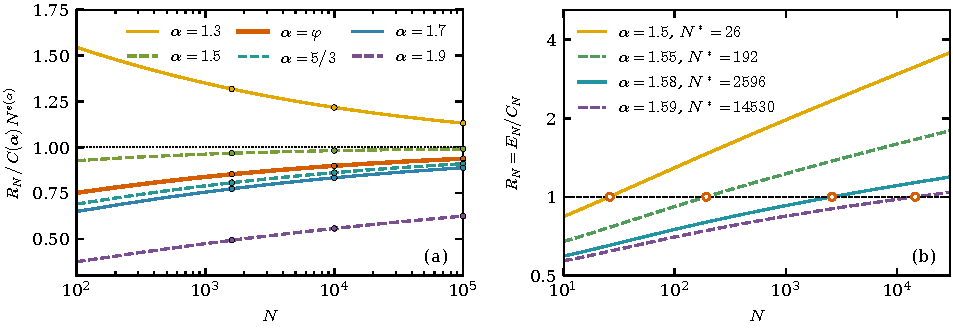
\includegraphics{figures/heavy}
\caption{Alternating runs with a stationary start. (a)
$R_N/(C(\alpha)N^{e(\alpha)})$ for even $N$ from $100$ to $10^5$, with the
entries of Table~\ref{tab:heavy} as dots. (b) $R_N$ for
$\alpha=1.5,1.55,1.58,1.59$ below $\varphi$. Each curve crosses $1$ once on
$10\le N\le3\cdot10^4$, at $N^*(\alpha)$ (circles).}
\label{fig:heavy}
\end{figure}

\begin{corollary}[the golden-ratio exponent]\label{cor:golden}
Let $1<\alpha<2$ and $e(\alpha)=1-\alpha+1/\alpha$. If
$\Prob(D\ge N)\sim c_DN^{-\beta_D}$ with $c_D,\beta_D>0$, then
$R_N\sim c_DN^{1/\alpha-\beta_D}/(4I_\alpha(2\mu)^{1/\alpha})$. In particular
$R_N\sim C(\alpha)N^{e(\alpha)}$ for the stationary start and
$R_N\sim C_{\rm fr}(\alpha)N^{e(\alpha)-1}$ for the fresh start, where
\[
 C(\alpha)=\frac{\pi\bigl(K_\alpha\lvert\cos\frac{\pi\alpha}2\rvert
 \bigr)^{1/\alpha}}{4(\alpha-1)\Gamma(1+\frac1\alpha)\,
 \zeta(\alpha)^{1+1/\alpha}},\qquad
 C_{\rm fr}(\alpha)=(\alpha-1)\zeta(\alpha)\,C(\alpha).
\]
Since $e(\alpha)>0$ exactly when $\alpha<\varphi$, with a stationary start the
ends win for all large $N$ if $\alpha<\varphi$, and the center wins if
$\alpha>\varphi$. At $\alpha=\varphi$,
\[
 R_N\to C(\varphi)=\frac{\pi\varphi\bigl(\varphi\,\Gamma(\varphi^{-2})\lvert
 \cos\frac{\pi\varphi}2\rvert\bigr)^{1/\varphi}}{4\,\Gamma(\varphi)\,
 \zeta(\varphi)^{\varphi}}=0.7761317206\ldots,
\]
so the center still wins, by the factor $1/C(\varphi)=1.2884\ldots$ in the
limit. That $C(\varphi)<1$ needs no computation (see the proof). With a fresh
start $e(\alpha)-1<0$, and the center wins for every $1<\alpha<2$.
\end{corollary}

\begin{proof}
We prove the general formula, then read off the two starts, and then treat
$\alpha=\varphi$. By Proposition~\ref{prop:edge} and Theorem~\ref{thm:center}, with $h=N/2$, we
have $R_N=\Prob(D\ge N)/(2C_N)$, and this is asymptotic to
$c_DN^{-\beta_D}/(4I_\alpha(2\mu/N)^{1/\alpha})$, which is the general formula.
By Lemma~\ref{lem:stable}(iv),
$4I_\alpha(2\mu)^{1/\alpha}=4\Gamma(1+\frac1\alpha)\mu^{1/\alpha}/(\pi(K_\alpha\lvert\cos\frac{\pi\alpha}2\rvert)^{1/\alpha})$.
The fresh start has $c_D=1$ and $\beta_D=\alpha$, which gives
$C_{\rm fr}(\alpha)$. By Proposition~\ref{prop:edge} the stationary start has
$c_D=1/((\alpha-1)\mu)$ and $\beta_D=\alpha-1$, which gives $C(\alpha)$. Next,
$e(\alpha)=-(\alpha^2-\alpha-1)/\alpha$, and $\varphi$ is the positive root of
$\alpha^2-\alpha-1$. At $\alpha=\varphi$ we have $\alpha-1=1/\varphi$,
$1+1/\alpha=\varphi$ and $2-\alpha=\varphi^{-2}$. So
$K_\varphi=\varphi\,\Gamma(\varphi^{-2})$, and substituting these into
$C(\alpha)$ gives the closed form. To see that $C(\varphi)<1$, we use four
elementary bounds. Since $x^{-\varphi}$ is convex, the trapezoid rule
overestimates its integral over $[1,\infty)$, so
$\zeta(\varphi)-\frac12\ge1/(\varphi-1)=\varphi$. The minimum of $\Gamma$ on
$(0,\infty)$ is $0.8856\ldots$~\cite[Section~5.4(iii)]{dlmf}, so
$\Gamma(\varphi)\ge0.8856$. Since $\Gamma\le1$ on $[1,2]$,
$\Gamma(\varphi^{-2})=\Gamma(1+\varphi^{-2})\varphi^2\le\varphi^2$. Finally
$\frac\pi2<\frac{\pi\varphi}2<\frac{5\pi}6$, so
$\lvert\cos\frac{\pi\varphi}2\rvert\le\frac{\sqrt3}2$. Together these give
$C(\varphi)\le\pi\varphi(\sqrt3\varphi^3/2)^{1/\varphi}/(4\cdot0.8856\,(\varphi+\frac12)^\varphi)=0.95136\ldots<1$.
\end{proof}

Corollary~\ref{cor:golden} is the lattice form, with its constant, of the
heuristic of~\cite[Section~6.2.1.3, Eq.~(6.49)]{wlh2016}. The approach to $C(\varphi)$ is
slow. At $\alpha=\varphi$ we have $R_{10^5}/C(\varphi)=0.938$, and $R_N$
increases at every even $N$ from $10$ to $10^5$ (Table~\ref{tab:heavy} and
Figure~\ref{fig:heavy}). At the value $\alpha=5/3$ of L\'evy-walk models of
heat conduction~\cite{cdp2005,dsd2013,zdk2015}, $R_N\sim C(5/3)N^{-1/15}$ with
$C(5/3)=0.8351$.

\begin{remark}[broadened side peaks]\label{rem:humps}
With velocity fluctuations the ballistic side peaks of a L\'evy walk broaden
into humps. If the speed is
redrawn at each collision, the humps have width of order $t$ and height of
order $t^{-\alpha}$, and if it fluctuates during each flight, they have width
of order $t^{1/2}$ and height of order
$t^{1/2-\alpha}$~\cite[Table~I]{dzh2012}. As a heuristic, matching these heights with the
height $t^{-1/\alpha}$ of the central
peak~\cite[Section~6.2.1.3, Eq.~(6.49)]{wlh2016} gives $\alpha=1$ in the first case, so the center wins for
every $1<\alpha<2$, and in the second case the root
$\alpha=(1+\sqrt{17})/4=1.28\ldots$ of $\alpha^2-\alpha/2-1=0$. The golden
ratio belongs to the unbroadened peaks, which our lattice walk has.
\end{remark}

We turn to the other exponents. Table~\ref{tab:outcomes} collects them. For
$\alpha\ge2$ the sums $\tau_m$ have a Gaussian limit, and the center wins
with either start.

\begin{table}[t]
\centering\footnotesize
\setlength{\tabcolsep}{4pt}
\begin{tabular}{@{}lllll@{}}
\toprule
$\alpha$ & start & center $C_N$ & ratio $R_N$ & status\\
\midrule
$\alpha>2$ & stationary & $\sim\sqrt{2\mu/(\pi vN)}$ & $\sim C_2(\alpha)N^{3/2-\alpha}\to0$ & Theorem~\ref{thm:alpha2}(a)\\
$\alpha=2$ & stationary & $\sim\sqrt{2\mu/(\pi N\log N)}$ & $\sim\sqrt{\pi\log N/(8\zeta(2)^3N)}\to0$ & Theorem~\ref{thm:alpha2}(b)\\
$1<\alpha<2$ & stationary & $\sim2I_\alpha(\mu/h)^{1/\alpha}$ & $\sim C(\alpha)N^{e(\alpha)}$ & Corollary~\ref{cor:golden}\\
$1<\alpha<2$ & fresh & $\sim2I_\alpha(\mu/h)^{1/\alpha}$ & $\sim C_{\rm fr}(\alpha)N^{e(\alpha)-1}\to0$ & Corollary~\ref{cor:golden}\\
$\alpha=1$ & fresh & $\approx2/(\pi^2\tilde m_h)$ & $\approx\pi^2\tilde m_h/(8h)\sim\pi^2/(8\log N)$ & heuristic, not proved (Remark~\ref{rem:other})\\
$0<\alpha<1$ & fresh & $\sim\frac2\pi\tan\frac{\pi\alpha}2\cdot\frac1N$ & $\sim\frac{\pi}{4\tan(\pi\alpha/2)}\,N^{1-\alpha}\to\infty$ & Theorem~\ref{thm:lamperti}\\
\bottomrule
\end{tabular}
\caption{The center and the ratio $R_N=E_N/C_N$ for each exponent. The center
wins when $R_N\to0$ and the ends win when $R_N\to\infty$. For $\alpha\ge2$ the
center formula holds for every a.s.\ finite first run, and a fresh start also
gives $R_N\to0$.}
\label{tab:outcomes}
\end{table}

\begin{theorem}[$\alpha\ge2$]\label{thm:alpha2}
Let $D$ be any a.s.\ finite first run, and let $N\to\infty$ over even $N$.
\begin{enumerate}[(a)]
\item Let $\alpha>2$ and
$v=\Var\xi=2\zeta(\alpha-1)-\zeta(\alpha)-\zeta(\alpha)^2$. Then
$C_N\sim\sqrt{2\mu/(\pi vN)}$. With the stationary start
$R_N\sim C_2(\alpha)N^{3/2-\alpha}$, where
$C_2(\alpha)=\sqrt{\pi v/(2\mu)}\big/(2(\alpha-1)\mu)$.
\item Let $\alpha=2$, so that $\mu=\zeta(2)$ and $\E\xi^2=\infty$. Then
$(\tau_m-m\mu)/\sqrt{m\log m}$ converges in law to the standard normal law,
and $C_N\sim\sqrt{2\mu/(\pi N\log N)}$. With the stationary start
$R_N\sim\sqrt{\pi\log N/(8\zeta(2)^3N)}$.
\end{enumerate}
In both cases $R_N\to0$ with the fresh start too.
\end{theorem}

The exponent of $R_N$ is continuous at $\alpha=2$, since
$e(2)=-\frac12=\frac32-2$. The proof of Theorem~\ref{thm:center} in
Appendix~\ref{app:heavy} is written so that it covers this theorem too, with
the normal law in place of the stable law
(Appendix~\ref{app:heavy-alpha2}).

The convergence is slow at $\alpha=2$. There $R_N$ divided by the leading
term in (b) is $0.885$ at $N=1600$ and $0.943$ at $N=10^5$. At $\alpha=3$
the ratio of $R_N$ to the leading term in (a) is $0.981$ at $N=16000$.

For $0<\alpha<1$ the runs have infinite mean, and only the fresh start makes
sense. Then $A_N/N$ has a limit law that is not concentrated at a point,
namely Lamperti's occupation-time
law~\cite{lamperti1958,godrecheluck2001}, with density
\[
 \ell_\alpha(y)=\frac{\sin\pi\alpha}{\pi}\,
 \frac{y^{\alpha-1}(1-y)^{\alpha-1}}{y^{2\alpha}+2y^\alpha(1-y)^\alpha
 \cos\pi\alpha+(1-y)^{2\alpha}}\qquad(0<y<1).
\]
So the center should be of order $1/N$. The next theorem is the local form
of this at the center.

\begin{theorem}[$0<\alpha<1$]\label{thm:lamperti}
Let $0<\alpha<1$, with a fresh start. As $N\to\infty$ over even $N$,
\[
 NC_N\to\ell_\alpha(\tfrac12)=\frac2\pi\tan\frac{\pi\alpha}2 .
\]
Hence $R_N\sim\frac{\pi}{4\tan(\pi\alpha/2)}N^{1-\alpha}\to\infty$.
\end{theorem}

In words, for $\alpha<1$ the center is an ordinary bin of size about $1/N$,
while the end has the much larger probability $\frac12N^{-\alpha}$ that the
first run goes right and lasts all $N$ steps. So the ends win for every $\alpha<1$.
For the continuum L\'evy walk with $0<\alpha<1$, the ballistic regime,
Froemberg et al.~\cite{fsbz2015} find the asymptotic densities.

\paragraph{Idea of the proof.}
Now $\tau_m$ is of order $m^{1/\alpha}$ with no centering, and the number of
runs of each sign is no longer concentrated, so the sum over it becomes an
integral (Appendix~\ref{app:heavy-lamperti}). The proof does not use
Lamperti's theorem.

Here too the convergence is slow near $\alpha=1$. At $N=16000$ the ratio of
$NC_N$ to its limit is $1.042$, $1.001$, $0.928$ and $0.554$ for
$\alpha=0.3$, $0.5$, $0.7$ and $0.9$. We do not prove the local limit at
bins other than the center.

\begin{remark}[the exponent $\alpha=1$ and the fresh start]\label{rem:other}
With a fresh start the threshold is $\alpha=1$. The ends win for $\alpha<1$
by Theorem~\ref{thm:lamperti}, and the center wins for $\alpha>1$ by
Corollary~\ref{cor:golden} and Theorem~\ref{thm:alpha2}. At $\alpha=1$ we
only have a heuristic. Suppose we repeat the proof of
Theorem~\ref{thm:center} with a skewed Cauchy limit, the centering
$m(H_{m+1}-1)$, and the density $1/\pi^2$ at $0$ of the difference of two
copies of the limit. This suggests the row of Table~\ref{tab:outcomes},
namely $R_N\approx\pi^2\tilde m_h/(8h)\sim\pi^2/(8\log N)$, where
$\tilde m_h$ solves $m(H_{m+1}-1)=h$. We have not controlled the error
terms, so the claim that the center wins by a logarithm at $\alpha=1$ is not
proved. The computed $R_N$ divided by $\pi^2\tilde m_h/(8h)$ is $0.796$,
$0.850$ and $0.886$ at $N=1600$, $10^4$ and $10^5$.
\end{remark}

We do not know a rate in Theorem~\ref{thm:center}, whether $R_N$ is monotone
with a single sign change of $R_N-1$, how to make the case $\alpha=1$
rigorous, or the full shape of $P_N$ for heavy-tailed runs.

\section{Aging walks}\label{sec:aging}

In this section the walk remembers its age. After its first step it switches
direction at step $k\ge2$ with probability $c/k$, independently of the past,
where $0<c<2$. So the walk switches less and less often, and the expected
number of switches in $N$ steps is $c(H_N-1)$, which is about $c\log N$. With
a fair first step, $A_N/N$ converges in law to
$\mathrm{Beta}(c,c)$~\cite[Example~1.1 and Theorem~1.4]{ds2007},
\cite[Theorem~1]{ev2018}. At finite $N$ the first step
matters. We first give one exact law behind all the ties, then fix the first
step, pass to $d$ states, and return to the fair first step.

We write $\Prob_+$ for the law given $X_1=+1$, as in
Section~\ref{sec:notation}, and $X_N$ for the last step. A path is a sequence
$x\in\{\pm1\}^N$, and it switches at time $t\ge2$ if $x_t\ne x_{t-1}$. Step
$k\ge2$ contributes the factor $c/k$ to the probability of a path if the path
switches there, and $1-c/k$ otherwise. So relative to no switch, a switch at
time $t$ multiplies the probability of a path by the odds
\[
 \omega_t=\frac{c/t}{1-c/t}=\frac{c}{t-c}\qquad(t\ge2),
\]
and
\begin{equation}\label{eq:aging-path}
 \Prob_+(X=x)=\prod_{k=2}^N\Bigl(1-\frac ck\Bigr)\prod_{t:\,x_t\ne x_{t-1}}\omega_t
 \qquad(x_1=+1).
\end{equation}
Each $\omega_t$ is positive and continuous on $(0,2)$, increases strictly in
$c$, and tends to $0$ as $c\downarrow0$.

\subsection{Drawing afresh or repeating}\label{sec:aging-urn}

All the exact laws of this section come from one chain, which works for every
weight. Fix $d\ge2$ and $\theta>0$, and let $Y_1,Y_2,\dots$ be the following
chain on $\{1,\dots,d\}$. At step $t\ge1$, with probability
\[
 f_t=\frac{d\theta}{d\theta+t-1}
\]
the state $Y_t$ is drawn afresh, uniformly from the $d$ states, and otherwise
$Y_t=Y_{t-1}$ (so $Y_1$ is uniform, since $f_1=1$). In other words, at
step $t\ge2$ the chain moves to each other state with probability
$\theta/(d\theta+t-1)$. This is the mechanism of the conservative random walk
of Engl\"ander and Volkov~\cite{ev2022}, who redraw a direction in
$\mathbb Z^d$ with probability $p_n$ and study recurrence and scaling limits.
Let $M_T$ be the vector of visit counts of $Y_1,\dots,Y_T$, and write
$x^{(m)}=x(x+1)\cdots(x+m-1)$.

\begin{proposition}[fresh or repeat]\label{prop:aging-urn}
For every $T\ge1$, every composition $m$ of $T$ into $d$ nonnegative parts and
every state $j$,
\begin{equation}\label{eq:aging-urn}
 \Prob(M_T=m,\,Y_T=j)=\frac{m_j}{T}\,Q_T(m),\qquad
 Q_T(m)=\frac{T!}{(d\theta)^{(T)}}\prod_{i=1}^d\frac{\theta^{(m_i)}}{m_i!} .
\end{equation}
So $M_T$ has the law $Q_T$ of the counts in P\'olya's urn with $d$ colors and
initial weight $\theta$ on each color. For $d=2$ and even $T$,
\begin{equation}\label{eq:aging-urn-ratio}
 \frac{\Prob(M_T=(T/2,T/2))}{\Prob(M_T=(T,0))}
 =\binom{T}{T/2}\prod_{i=0}^{T/2-1}\frac{\theta+i}{\theta+T/2+i},
\end{equation}
which increases strictly in $\theta$ and equals $1$ exactly at $\theta=1$.
\end{proposition}

In words, the chain repeats its last state where the urn repeats a uniformly
chosen earlier draw, and at each fixed time this makes no difference to the
counts or to the last state. The whole law is explicit on both sides of the
tie (Figure~\ref{fig:aging}).

\begin{figure}[t]
\centering
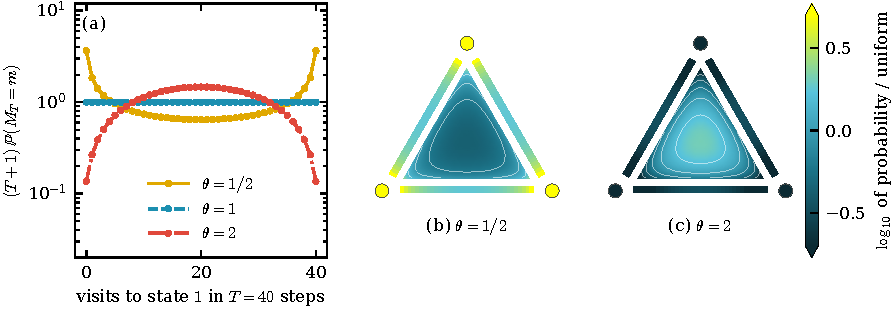
\includegraphics[width=\textwidth]{figures/aging}
\caption{The exact law~\eqref{eq:aging-urn} of the counts of the chain that
draws afresh or repeats. (a) Two states and $T=40$, as a multiple of the
uniform law. The law is flat at $\theta=1$, the ends are the most likely bins
for $\theta=\frac12$, and the center is for $\theta=2$. (b), (c) Three states
and $T=36$ on the simplex of visit fractions, colored by the probability of a
bin relative to the uniform law. The triangle holds the bins that use all three
states, the bands hold the bins that use two, and the disks are the bins that
use one. The thin lines are level lines. For $\theta=\frac12$ a corner is
$9.6$ times as likely as under the uniform law and the center $0.43$ times.
For $\theta=2$ the numbers are $0.035$ and $2.1$.}
\label{fig:aging}
\end{figure}

\begin{proof}
We use induction on $T$. For $T=1$ both sides of~\eqref{eq:aging-urn} are
$\frac1d$ when $m=e_j$ and $0$ otherwise. Let $T\ge2$ and suppose
\eqref{eq:aging-urn} holds for $T-1$. If $m_j=0$ both sides vanish. Otherwise
put $m'=m-e_j$. Summing~\eqref{eq:aging-urn} over the last state gives
$\Prob(M_{T-1}=m')=Q_{T-1}(m')$. A fresh draw gives $j$ with probability
$\frac1d$ whatever the last state was, and a repeat gives $j$ only when the
last state was $j$ (this is why the induction carries the last state along
with the counts). So
\[
 \Prob(M_T=m,\,Y_T=j)
 =\frac{f_T}{d}\,Q_{T-1}(m')+(1-f_T)\,\frac{m_j-1}{T-1}\,Q_{T-1}(m')
 =\frac{\theta+m_j-1}{d\theta+T-1}\,Q_{T-1}(m') .
\]
On the other hand
$Q_T(m)=Q_{T-1}(m')\cdot\frac{T}{m_j}\cdot\frac{\theta+m_j-1}{d\theta+T-1}$ by
the definition of $Q_T$. This gives~\eqref{eq:aging-urn}. Summing over $j$
gives $\Prob(M_T=m)=Q_T(m)$, and the ratio~\eqref{eq:aging-urn-ratio} is
$Q_T(T/2,T/2)/Q_T(T,0)$ with
$\theta^{(T)}=\theta^{(T/2)}(\theta+T/2)^{(T/2)}$. Each factor
$(\theta+i)/(\theta+T/2+i)$ increases strictly in $\theta$, and at
$\theta=1$ the product is $(T/2)!^2/T!$.
\end{proof}

The law of the counts alone is known. Dietz, Lippitt and
Sethuraman~\cite[Theorem~2.18]{dls2023} show that the moments of the limit
law of the chains of~\cite{ds2007} are occupation probabilities at finite $N$
of a second chain. In the case of a Dirichlet limit that second chain is
$Y$, with the uniform law in the role of their $\mu$ and $d\theta$ in the role
of their $\theta$. The limit is then the Dirichlet law with every parameter
$\theta$~\cite[Theorem~1.4]{ds2007}, and its moments give $Q_T$.
Engl\"ander and Volkov work it out in Chapter~7 of their
\hyperref[fn:evdraft]{March 18, 2024 draft}. For two states and an integer weight $\theta$
they prove~\eqref{eq:aging-urn}, with the last state, for every
$T$~\draftloc{Theorem~7.2, pp.~138--139}, and they credit this result to E.~Crane.
What the proposition adds is the joint law with the last state for $d\ge3$
states, and for a weight $\theta$ that is not an integer. As $T\to\infty$,
\eqref{eq:aging-urn} turns into the joint limit of the fractions of time and
the current state found by Bouguet and Cloez~\cite[Proposition~4.1]{bc2018},
in which the Dirichlet law is size-biased by the coordinate of the current
state.

\begin{remark}\label{rem:aging-feller}
Here is another way to see the law of the counts in
Proposition~\ref{prop:aging-urn} (but not the joint law with the last state).
The fresh draws
cut $Y_1,\dots,Y_T$ into runs, and each run gets a uniform state. The urn can
be run in the same way, as a Chinese restaurant process in which each table
gets a uniform color. There a table is opened with the same probabilities
$f_t$. The lengths of the runs are the spacings between the successes of
independent trials with success probabilities $f_t$. It is a classical
fact (the Feller coupling, see~\cite{abt2003}) that the multiset of these spacings has
the same law as the multiset of the table sizes (the two ordered lists do not).
The proof in~\draftloc{Section~7.4}, like
Proposition~\ref{prop:aging-urn}, instead goes through the last state. We
checked~\eqref{eq:aging-urn} in exact arithmetic for four values of $\theta$,
with $T\le7$ for $d=2,3$ and $T\le5$ for $d=4$
(\texttt{verify\_aging\_urn.py}).
\end{remark}

\subsection{A fixed first step}

Here the walk starts with a step $+1$.

\begin{proposition}[two states, fixed first step]\label{prop:aging-two}
Let $N\ge2$ and let the first step be $+1$.
\begin{enumerate}[(a)]
\item At $c=1$, for $1\le s\le N$,
\[
 \Prob_+(A_N=s,\,X_N=+1)=\frac{s-1}{N(N-1)},\qquad
 \Prob_+(A_N=s,\,X_N=-1)=\frac{N-s}{N(N-1)}.
\]
So $A_N$ is uniform on $\{1,\dots,N\}$.
\item For $1\le s\le N-1$ the ratio $\Prob_+(A_N=s)/\Prob_+(A_N=N)$ increases
strictly in $c\in(0,2)$, and it equals $1$ exactly at $c=1$.
\end{enumerate}
\end{proposition}

For $c<1$ the end bin is the most likely
bin, and for $c>1$ it is the least likely of the bins $1,\dots,N$ (bin $0$
has probability $0$).

\begin{proof}
(a) At $c=1$, the shifted chain $Y_t=X_{t+1}$ is the chain of
Proposition~\ref{prop:aging-urn} with $d=2$, $\theta=1$ and uniform first
state. Apply~\eqref{eq:aging-urn} at $T=N-1$ with counts $(s-1,N-s)$,
where $Q_{N-1}=1/N$, then sum over the last state.

(b) We write the ratio as a sum over paths. Only the path with every step
$+1$ has $A_N=N$, and it never switches. So $\Prob_+(A_N=N)$ is the first
product in~\eqref{eq:aging-path}, and dividing by it leaves
\begin{equation}\label{eq:aging-ratio}
 \frac{\Prob_+(A_N=s)}{\Prob_+(A_N=N)}
 =\sum_{x}\ \prod_{t:\,x_t\ne x_{t-1}}\omega_t ,
\end{equation}
where the sum is over the paths $x$ with $x_1=+1$ and $s$ steps equal to
$+1$. For example, for $N=3$ and $s=2$ the paths are $(+,+,-)$ and $(+,-,+)$,
and the ratio is $\omega_3+\omega_2\omega_3$. For $1\le s\le N-1$ there is
such a path, and each of them switches at least once. So the right side is a
sum of products of the $\omega_t$ with at least one factor each. Each
$\omega_t$ is positive and increases strictly in $c$, so the sum does too. By
(a) it equals $1$ at $c=1$.
\end{proof}

After a shift of one step, part (a) is the exercise
in~\cite[Section~3.1, footnote~1]{evw2020}. That footnote also says that the fact
can be related to P\'olya urns (the authors credit M.~Bal\'azs) and that a
more general connection of their model with P\'olya urns will appear in a
later paper.
That connection is developed in Chapter~7 of the dated draft, and after the same
shift part (a), with the last state, is~\draftloc{Claim~7.1}. So part (a)
is not new. What we add for
two states is part (b), and the count law also follows
from~\cite[Theorem~2.18]{dls2023} (Section~\ref{sec:aging-urn}). Both parts of
Proposition~\ref{prop:aging-two} are also proved in Lean
(Section~\ref{sec:verify}).

\subsection{\texorpdfstring{$d$}{d} states}

The same thing happens for a chain on $d$ states that leaves its current
state for each other state at the same aging rate. Fix $d\ge2$ and $\theta$
with $0<\theta<d/(d-1)$. The chain $X_1,X_2,\dots$ on $\{1,\dots,d\}$ starts at
$X_1=1$. At step $k\ge2$ it moves to each of the other $d-1$ states with
probability $\theta/(k+d-2)$, and it stays with probability
$1-(d-1)\theta/(k+d-2)$. The condition on $\theta$ says that the probability
of staying is positive at every step $k\ge2$. Let
$L_N=(L_N(1),\dots,L_N(d))$ be the vector of visit counts, namely
$L_N(i)=\#\{k\le N:X_k=i\}$. Its values are the compositions
$n=(n_1,\dots,n_d)$ of $N$ into $d$ nonnegative parts with $n_1\ge1$. There
are $\binom{N+d-2}{d-1}$ of them (subtract one from $n_1$). We call them
bins. The corner $Ne_1$, where $e_i$ is the $i$-th unit vector, is the bin of
the chain that never moves.

For such chains Dietz and Sethuraman~\cite[Theorem~1.4]{ds2007} proved that
the fractions of time converge in law to the Dirichlet law with every
parameter $\theta$, which is uniform on the simplex exactly at $\theta=1$.
After a shift of the time index by $d-2$, their chain and ours have the same
transition probabilities at every time $n\ge d+1$, and after one common fresh
draw the two chains agree, so their fractions of time have the same limit. At
$\theta=1$, part~(a) of the theorem below is an exact finite-$N$ form of this
limit.

\begin{theorem}[$d$ states]\label{thm:aging-d}
Let $d\ge2$, $0<\theta<d/(d-1)$ and $N\ge2$.
\begin{enumerate}[(a)]
\item At $\theta=1$, for every bin $n$ and every state $j$,
\begin{equation}\label{eq:aging-d}
 \Prob(L_N=n,\,X_N=j)=\frac{n_j-\mathbf 1\{j=1\}}{(N-1)\binom{N+d-2}{d-1}} .
\end{equation}
So $L_N$ is uniform on the $\binom{N+d-2}{d-1}$ bins, the corner included.
\item For every bin $n\ne Ne_1$ the ratio $\Prob(L_N=n)/\Prob(L_N=Ne_1)$
increases strictly in $\theta$, and it equals $1$ exactly at $\theta=1$.
\end{enumerate}
\end{theorem}

In words, at $\theta=1$, given the counts, the
last state is distributed as the state at a uniformly chosen one of the steps
$2,\dots,N$ (the forced first visit to state $1$ is left out).
Below $\theta=1$ the corner is the most likely bin, and above it the corner
is the least likely.

\begin{proof}
(a) At $\theta=1$, $X_2$ is uniform and $Y_t=X_{t+1}$ is the chain
of Proposition~\ref{prop:aging-urn}. Its count vector is $L_N-e_1$, and
$Q_{N-1}=1/\binom{N+d-2}{d-1}$. Formula~\eqref{eq:aging-urn} gives
\eqref{eq:aging-d}, and summing over $j$ gives the uniform law.

(b) A path $x\in\{1,\dots,d\}^N$ with $x_1=1$ has probability
$\prod_{k=2}^N\bigl(1-\frac{(d-1)\theta}{k+d-2}\bigr)$ times the product of
the odds
\[
 \omega^{(d)}_t=\frac{\theta/(t+d-2)}{1-(d-1)\theta/(t+d-2)}
 =\frac{\theta}{t+d-2-(d-1)\theta}
\]
over the times $t\ge2$ with $x_t\ne x_{t-1}$. The denominator is positive and
decreases in $\theta$, so each $\omega^{(d)}_t$ increases strictly in
$\theta$. Only the constant path has counts $Ne_1$. So
$\Prob(L_N=n)/\Prob(L_N=Ne_1)$ is the sum of the products of the odds over
the paths with counts $n$. For a bin $n\ne Ne_1$ there is such a path, and
each of them moves at least once. Hence the ratio increases strictly in
$\theta$, and by (a) it equals $1$ at $\theta=1$.
\end{proof}

\begin{remark}\label{rem:aging-d}
For $d=2$ the chain switches at step $k$ with probability $\theta/k$, so
Theorem~\ref{thm:aging-d} with $\theta=c$ is
Proposition~\ref{prop:aging-two}, and~\eqref{eq:aging-d} reads
$(s-1)/(N(N-1))$ for $j=1$ and $n=(s,N-s)$.

By Proposition~\ref{prop:aging-urn}, $(L_N-e_1,X_N)$ has the law of
the counts and last color of $N-1$ draws from P\'olya's urn with one ball of
each color. This is an identity at each fixed time, not an identity of path
laws. For example, with $d=2$ and $N=4$ the chain path $1,1,2,2$ has
probability $1/8$, while the urn draws $1,2,2$ have probability $1/12$.
For two states Engl\"ander and Volkov call this relation
mimicking~\draftloc{Definition~7.1 and Lemma~7.1}, and they show with an
example of three steps that the coin-turning walk and the urn have different
path laws~\draftloc{Example~7.1}. Also, at $\theta=1$ the chain moves at
step $k$ with probability $(d-1)/(k+d-2)$, independently over $k$. This is
the probability that customer $k$ opens a new table in the Chinese restaurant
process with parameter $d-1$. So the expected number of moves in $N$ steps at
the tie is $\sum_{k=2}^N\frac{d-1}{k+d-2}=(d-1)\log N+O(1)$, which has the
same order, $\log N$, as the number of turns at the crossing from the corners
to the center for $d$ directions and runs of geometric length~\cite{paperB}.

We checked~\eqref{eq:aging-d}, and the strict ordering in (b) along the five
values $\theta=\frac12,\frac9{10},1,\frac{11}{10},\frac54$, in exact
rational arithmetic for $d=2,3,4$ and $2\le N\le8$
(\texttt{verify\_aging.py}).
\end{remark}

\subsection{A fair first step}

We return to two states and let the first step be fair. Then both ends can be
reached, and $E_N=\Prob(A_N=N)=\frac12\prod_{k=2}^N(1-c/k)$. Changing the sign
of every step preserves the law of the walk and sends $A_N$ to $N-A_N$. So
\begin{equation}\label{eq:aging-fair}
 \Prob(A_N=s)=\tfrac12\bigl(\Prob_+(A_N=s)+\Prob_+(A_N=N-s)\bigr),\qquad
 E_N=\tfrac12\Prob_+(A_N=N),
\end{equation}
since $\Prob_+(A_N=0)=0$.

\begin{proposition}[fair first step]\label{prop:aging-fair}
Let $N\ge2$ and $1\le s\le N-1$, with a fair first step.
\begin{enumerate}[(a)]
\item At $c=1$, $\Prob(A_N=s)=\frac1N$ and $E_N=\frac1{2N}$.
\item The ratio $\Prob(A_N=s)/E_N$ is continuous and strictly increasing in
$c\in(0,2)$. It tends to $0$ as $c\downarrow0$ and equals $2$ at $c=1$. So
there is exactly one $c$ in $(0,2)$ with $\Prob(A_N=s)=E_N$, and it is less
than $1$.
\end{enumerate}
\end{proposition}

For even $N$ we write $c_N$ for the crossing in (b) with $s=h=N/2$, so that
$C_N=E_N$ exactly at $c=c_N$. In words, at $c=1$ every interior bin still has
probability $\frac1N$, and the two ends share the probability $\frac1N$ that
the fixed start gave to one end.
Related fair-start formulas for switch probabilities $1/(n+a)$ appear
in~\draftloc{Section~5.7, p.~76}. Its first displayed family is
twice a normalized law. We do not use that formula, and derive (a) from
the averaging identity~\eqref{eq:aging-fair}.

\begin{proof}
(a) This follows from~\eqref{eq:aging-fair} and
Proposition~\ref{prop:aging-two}(a). (b) By~\eqref{eq:aging-fair} the ratio
is the sum of the right sides of~\eqref{eq:aging-ratio} for $s$ and for
$N-s$. Both are finite sums of products of at least one $\omega_t$. So the
ratio is continuous and strictly increasing, and it tends to $0$ as
$c\downarrow0$. By (a) it equals $2$ at $c=1$. Hence it equals $1$ exactly
once, at some $c<1$.
\end{proof}

How far below $1$ is $c_N$? The end is of order $N^{-c}$ and the center is of
order $1/N$, so they meet when $N^{1-c}$ is about $2$.

\begin{proposition}[the fair-start crossing]\label{prop:aging-expansion}
For even $N\to\infty$,
\[
 c_N=1-\frac{\log2}{\log N+\gamma+2-2\log2}+O\bigl((\log N)^{-3}\bigr),
\]
where $\gamma$ is Euler's constant.
\end{proposition}

\paragraph{Idea of the proof.}
A monotonicity argument first traps $c_N$ within $O(1/\log N)$ of $1$, so an expansion at $c=1$
applies. The end is explicit, namely
$E_N=\Gamma(N+1-c)/(2\Gamma(2-c)\Gamma(N+1))$, which is
$N^{-c}/(2\Gamma(2-c))$ with relative error $O(1/N)$. For the center we prove
a local limit theorem with a rate, namely $NC_N=d_c+O(\sqrt{\log N/N})$ uniformly
for $c\in[c^{(3)},1]$, where $c^{(3)}=(9-\sqrt{57})/2\approx0.725$ and $d_c=4^{1-c}/\mathrm B(c,c)$ is the density of
$\mathrm{Beta}(c,c)$ at $\frac12$. So
$\log(C_N/E_N)=(c-1)\log N+\Theta(c)+O(\sqrt{\log N/N})$ with
$\Theta(c)=\log(2\Gamma(2-c)d_c)$. Here $\Theta(1)=\log2$ and
$\Theta'(1)=\gamma+2-2\log2$, and solving for the zero gives the expansion.
The proof is in Appendix~\ref{app:aging}. There $C_N$ is an average of
explicit numbers over the law of the time of the $h$-th step $+1$
(Lemma~\ref{lem:D-average}). The local limit theorem comes from a coupling of
the walk with the chain of Proposition~\ref{prop:aging-urn} with $d=2$ and
$\theta=c$, whose counts are a mixture of binomial laws with a
$\mathrm{Beta}(c,c)$ parameter (Proposition~\ref{prop:D-llt}).

The error term decays only like $(\log N)^{-3}$, but the expansion is
already accurate at moderate $N$. The computed crossing at $N=200$ is
$c_{200}=0.8925$, against $0.8932$ from the expansion without its error term. The constant in
the error term is not computed.

\section{Verification}\label{sec:verify}

{\sloppy
This section says how the numbers in this paper were computed and which
results are also proved in Lean. All computations are in Python. The values of $R_N$ in Table~\ref{tab:heavy}
were computed in two ways, both from Proposition~\ref{prop:tworenewal},
namely by its formula and by a spectral method that reads each factor off as
a Taylor coefficient of a generating function. For small $N$ they were also
checked against a recursion on the first run and a sum over all run
compositions, which do not use Proposition~\ref{prop:tworenewal}. The aging
probabilities, and with them the crossing $c_{200}$, were computed in three
ways, namely by a forward recursion, from transfer matrices at roots of unity,
and from the sums over paths in~\eqref{eq:aging-ratio}. In exact rational
arithmetic $C_{200}-E_{200}$ is negative at $c_{200}-10^{-6}$ and positive at
$c_{200}+10^{-6}$.

No proof in this paper rests on a computation. The tables,
the figures and the numbers quoted outside the proofs rest on computation
alone. The script \texttt{verify\_heavy\_runs.py} recomputes the numbers of
Section~\ref{sec:heavy} and Appendix~\ref{app:heavy}, the script \texttt{verify\_aging.py}
those of Section~\ref{sec:aging} and Appendix~\ref{app:aging}, and
\texttt{verify\_aging\_urn.py} checks Proposition~\ref{prop:aging-urn} in exact arithmetic for
two, three and four states. The numbers in the caption of
Figure~\ref{fig:aging} come from \texttt{figures/make\_aging\_figure.py}.

Many statements of this paper are also proved in Lean~4.33.1 with Mathlib at commit
\texttt{0df444a360ea}, in the folder \nolinkurl{kagey-problems/problem131/lean/PaperD}, which
is shared with an earlier version of this work. The file \nolinkurl{MAP.md} there lists each
statement of this paper by its label, with its Lean names, its status in Lean and the source of
each classical input. The kernel checks every proof, and every theorem depends only on the
axioms \texttt{propext}, \texttt{Classical.choice} and \texttt{Quot.sound}.
The statement-by-label table in \nolinkurl{MAP.md} and the detailed table
\nolinkurl{coverage_F.tex} record the coverage and its qualifications. Some proofs use six classical
results, which Lean states as named hypotheses, and nothing else is assumed. These are the local
limit theorem of Gnedenko (GN)~\cite[Theorem~4.2.1]{ibragimovlinnik1971}, the expansion of
$\mathrm{Li}_s(e^{-v})$ near $v=0$ (POLY)~\cite[25.12.12]{dlmf}, the continuity theorem of
L\'evy (LEVY) and Fourier inversion for an integrable characteristic function
(FI)~\cite[Section~XV.3]{feller1971}, the continuity theorem for Laplace transforms
(LAP)~\cite[Section~XIII.1]{feller1971} and the uniqueness theorem of Lerch for Laplace
transforms (LERCH)~\cite[Chapter~II]{widder1941}.



One proof in Lean differs from ours. In Step~4 of the proof of Theorem~\ref{thm:lamperti},
Lean finds $\int_0^\infty tg(t)^2\,dt$ from $\E G^{i\tau}$ by Parseval's identity for the
density of $\log G$, so it does not identify the law of $G_1/(G_1+G_2)$. Lean does not
formalize the six classical results, Theorem~\ref{thm:alpha2},
Remarks~\ref{rem:humps}, \ref{rem:aging-feller} and~\ref{rem:other}, or
the numbers that rest on computation.
\par}

\paragraph{Open questions.}
For the heavy-tailed walk, a rate in Theorem~\ref{thm:center} remains open.
So does monotonicity of $E_N/C_N$ in $N$, which would give uniqueness of a
crossover size when the two probabilities exchange order.


\paragraph{Acknowledgments.} I thank Peter Kagey for posing the problem and
Aidan Deshong for insightful conversations.

\section*{A note on the use of AI}
I wrote the original draft and its mathematics. I used Claude Opus 5.5
(Anthropic) for revision and proof checking, and later used OpenAI Codex to
shorten the exposition and check references. The latter revision includes
the title, the derivations from the urn law and the verification discussion.
AI tools generated the Lean files and parts of the verification code, which
I reviewed against the paper. Section~\ref{sec:verify} states what Lean
proves and which classical results it takes as hypotheses. I checked the
revisions and take responsibility for the contents of the paper.

\appendix
\section{Proofs for Section~\ref{sec:heavy}}\label{app:heavy}

Sections~\ref{app:heavy-setting} to~\ref{app:heavy-alpha2} treat $\alpha>1$ and prove
Theorems~\ref{thm:center} and~\ref{thm:alpha2} together.
Section~\ref{app:heavy-lamperti} treats $0<\alpha<1$ and proves
Theorem~\ref{thm:lamperti}.

We use the notation of Section~\ref{sec:heavy}, with $\tau_0=0$. For a first run $D$ let
$\tau^D_m=D+\tau'_{m-1}$, where $(\tau'_m)$ is an independent copy of $(\tau_m)$, and
$\tau^D_0=0$. Then $u^D_m(k)=\Prob(\tau^D_m=k)$ and
$q^D_m(k)=\Prob(\tau^D_{m-1}<k\le\tau^D_m)$. We find each of these by conditioning on
where the run before ends. For example, the $m$-th run covers level $k$ exactly when the
first $m-1$ runs end at some level $k-j$ with $j\ge1$ and the $m$-th run has length at
least $j$. In this way, for $m,k\ge1$,
\begin{equation}\label{eq:C-conv}
\begin{gathered}
q_m(k)=\sum_{j\ge1}\bar F(j)\,u_{m-1}(k-j),\qquad
q^D_{m+1}(k)=\sum_{j\ge1}\bar F(j)\,u^D_m(k-j),\\
u^D_m(k)=\sum_{\ell\ge1}\Prob(D=\ell)\,u_{m-1}(k-\ell).
\end{gathered}
\end{equation}
Here $u_0(k)=\mathbf 1\{k=0\}$. The sums $\tau_m$ and $\tau^D_m$ increase strictly in $m$.
So exactly one run covers a given level $k\ge1$, and at most one run ends there. Hence
$\sum_mq_m(k)=\sum_mq^D_m(k)=1$ and $\sum_mu_m(k)\le1$, $\sum_mu^D_m(k)\le1$. Also, the
first $m'$ runs reach level $k$ exactly when one of them covers it, so
$\sum_{m\le m'}q_m(k)=\Prob(\tau_{m'}\ge k)$, and in the same way
$\sum_{m\le m'}q^D_m(k)=\Prob(\tau^D_{m'}\ge k)$.

\subsection{The setting for \texorpdfstring{$\alpha>1$}{alpha > 1}}\label{app:heavy-setting}

Let $\alpha>1$, so that $\mu=\zeta(\alpha)<\infty$. The proof of the center asymptotics uses
the exponent only through the following three facts about a norming sequence $(a_m)$ of
positive numbers.
\begin{enumerate}[(F1)]
\item For $m\ge3$ we have $a_m=a(m)$, where $a(x)=c_ax^{\kappa}(\log x)^{\beta}$ on
$[3,\infty)$ with constants $c_a>0$, $0<\kappa<1$ and $\beta\ge0$.
\item The variables $(\tau_m-m\mu)/a_m$ converge in law to a variable $G$ that has a
bounded, uniformly continuous density $g$ with $g(z)\to0$ as $\lvert z\rvert\to\infty$.
With $z_{m,k}=(k-m\mu)/a_m$, the numbers
$\delta_m=\sup_k\lvert a_mu_m(k)-g(z_{m,k})\rvert$ tend to $0$, and
$\bar u=\sup_{m\ge1}\sup_ka_mu_m(k)$ is finite.
\item There is a constant $C_B$ such that $u_m(k)\le C_B\,m\,k^{-\alpha-1}$ for all
$m\ge1$ and $k\ge2m\mu$.
\end{enumerate}
The function $a$ in (F1) is increasing, and $a(\lambda x)/a(x)\to\lambda^\kappa$ as
$x\to\infty$, uniformly for $\lambda$ in a compact subset of $(0,\infty)$. So
$a_m\to\infty$ and $a_m/a_{m-1}\to1$. For $1<\alpha<2$ we take $a_m=m^{1/\alpha}$. Then
(F1) holds with $\kappa=1/\alpha$ and $\beta=0$, (F2) is Lemma~\ref{lem:stable}(ii)
and~(iii), and (F3) is Lemma~\ref{lem:C-bigjump} below. We write $\omega$ for the modulus
of continuity of $g$ and $\bar g(x)=\sup_{\lvert y\rvert\ge x}g(y)$. So
$\omega(\eta)\to0$ as $\eta\to0$ and $\bar g(x)\to0$ as $x\to\infty$.

\subsection{Two lemmas on renewal sums}

A sum of $m$ runs that is much larger than its mean is most likely made by a single long
run. The first lemma turns this into a local bound. Bounds of this kind are
classical in the big-jump domain~\cite{dds2008}. We include a short
proof to keep the paper self-contained.

\begin{lemma}\label{lem:C-bigjump}
Let $\alpha>1$. There is a constant $C_B=C_B(\alpha)$ such that
$u_m(k)\le C_B\,m\,k^{-\alpha-1}$ for all $m\ge1$ and $k\ge2m\mu$.
\end{lemma}

\begin{proof}
We split the event $\{\tau_m=k\}$ according to whether some run is long, namely at least
$y=k/r$, where $r>2$ is a constant that depends only on $\alpha$ and is chosen below. The
first part is small because one run takes a given value $\ell\ge y$ with probability at
most $\alpha y^{-\alpha-1}$. If no run is long, then $\tau_m$ is a sum of variables below $y$ whose mean is at most $k/2$,
and a Chernoff bound shows that such a sum rarely reaches $k$. Here $C$ depends only on
$\alpha$ and may change from line to line. Since $\mu\ge1$ we have $m\le k/2$.

\emph{One big jump.} By the mean value theorem
$\Prob(\xi=\ell)=\ell^{-\alpha}-(\ell+1)^{-\alpha}\le\alpha\ell^{-\alpha-1}$. Fix an
index $i$. Then
\[
\Prob(\tau_m=k,\,\xi_i\ge y)=\sum_{\ell\ge y}\Prob(\xi=\ell)\,\Prob(\tau_m-\xi_i=k-\ell)
\le\alpha y^{-\alpha-1}=\alpha r^{\alpha+1}k^{-\alpha-1},
\]
because the first factor is at most $\alpha y^{-\alpha-1}$ and the second factors add up
to at most $1$. The $m$ indices together give at most $\alpha r^{\alpha+1}mk^{-\alpha-1}$.

\emph{No big jump.} We may take $y\ge1$, since otherwise $\max_i\xi_i<y$ is impossible.
Let $x_0>0$ and $s\ge0$. For $0\le x\le s$ we have
$e^x\le1+x+\frac{x^2}2e^s$. We use this with $x=s\xi/y$ on the event $\{\xi<y\}$ and then
$1+x\le e^x$. This gives
$\E[e^{s\xi/y};\xi<y]\le\exp\bigl(\frac sy\E[\xi;\xi<y]+\frac{s^2e^s}{2y^2}\E[\xi^2;\xi<y]\bigr)$.
By independence and Markov's inequality for $e^{s\tau_m/y}$,
\begin{equation}\label{eq:C-chernoff}
\Prob\bigl(\tau_m\ge x_0,\ \max_{i\le m}\xi_i<y\bigr)
\le\exp\Bigl(-\frac{sx_0}y+m\Bigl(\frac sy\,\E[\xi;\xi<y]
+\frac{s^2e^s}{2y^2}\,\E[\xi^2;\xi<y]\Bigr)\Bigr).
\end{equation}
We take $x_0=k$. Since $\E[\xi;\xi<y]\le\mu$ and $k-m\mu\ge k/2$, the first two terms of
the exponent add up to at most $-\frac sy\cdot\frac k2=-sr/2$. So the exponent is at most
$-sr/2+\frac12r^2s^2e^s\,m\,k^{-2}\,\E[\xi^2;\xi<y]$. It remains to choose $s$ and $r$ so that the bound is at most $Cmk^{-\alpha-1}$. The
choice depends on how fast the truncated second moment grows, so there are three cases.

Let $1<\alpha<2$. Then $\E[\xi^2;\xi<y]\le\alpha\sum_{\ell<y}\ell^{1-\alpha}\le
Cy^{2-\alpha}$, so the exponent is at most $-sr/2+Cr^\alpha s^2e^sm/k^\alpha$. Take
$s=\frac12\log(k^\alpha/m)$, which is positive since $m\le k/2<k^\alpha$. Then
$e^sm/k^\alpha=e^{-s}$ and $s^2e^{-s}\le1$, so the second term is at most $Cr^\alpha$.
The first term is $-\frac r4\log(k^\alpha/m)$. So the probability is at most
$C(m/k^\alpha)^{r/4}$. We take $r=4+4/(\alpha-1)$, so that $r/4=1+1/(\alpha-1)$. Since
$m\le k$, the bound is at most
$C(m/k^\alpha)(k^{1-\alpha})^{1/(\alpha-1)}=Cmk^{-\alpha-1}$.

Let $\alpha>2$. Then $\E[\xi^2;\xi<y]\le\E\xi^2<\infty$, so the exponent is at most
$-sr/2+Cr^2s^2e^sm/k^2$. Take $s=\frac12\log(k^2/m)$, which is positive since $m<k^2$.
As before the probability is at most $C(m/k^2)^{r/4}$. With $r=4\alpha$ and $m\le k$
this is $C\,m\,m^{\alpha-1}k^{-2\alpha}\le Cmk^{-\alpha-1}$.

Let $\alpha=2$. Then $\E[\xi^2;\xi<y]\le2\sum_{\ell<y}\ell^{-1}\le2\log(ek)$, so the
exponent is at most $-sr/2+r^2s^2e^sm\log(ek)/k^2$. Take
$s=\frac12\log\frac{k^2}{m\log(ek)}$, which is positive since
$m\log(ek)\le\frac12k\log(ek)<k^2$. As before the probability is at most
$C(m\log(ek)/k^2)^{r/4}$. With $r=20$ and $m\le k$ this is at most
$Cmk^{-6}\log^5(ek)\le Cmk^{-3}$.

In each case the two bounds together give the lemma.
\end{proof}

\begin{lemma}\label{lem:C-firstpassage}
Let $\alpha>1$ and assume \textup{(F1)} and \textup{(F2)}. Let $D$ be any a.s.\ finite
first run. Then
\[
\sup_k\Bigl\lvert\frac{a_m}\mu q_m(k)-g(z_{m,k})\Bigr\rvert,\qquad
\sup_k\bigl\lvert a_mu^D_m(k)-g(z_{m,k})\bigr\rvert,\qquad
\sup_k\Bigl\lvert\frac{a_m}\mu q^D_{m+1}(k)-g(z_{m,k})\Bigr\rvert
\]
tend to $0$ as $m\to\infty$. For $m\ge2$, $\sup_kq_m(k)\le\mu \bar u/a_{m-1}$ and
$\sup_ku^D_m(k)\le \bar u/a_{m-1}$.
\end{lemma}

\begin{proof}
By \eqref{eq:C-conv}, $q_m$ and $u^D_m$ are sums of shifts of $u_{m-1}$ with total
weights $\sum_j\bar F(j)=\mu$ and $1$. Since $u_{m-1}(k)\le\bar u/a_{m-1}$, this gives the
two bounds for $m\ge2$.

For the limits we use that a shift by a bounded amount $j$ moves the point $z_{m,k}$ only
by $O(1/a_m)$, and that $g$ is uniformly continuous. So the local limit for $u_{m-1}$
passes to these sums. We give the details for $q_m$. Fix $J\ge1$ and $Z>0$, put
$\sigma_J=\sum_{j>J}\bar F(j)$ and write $z=z_{m,k}$. We compare term by term the two sums
\[
a_{m-1}q_m(k)=\sum_{j\ge1}\bar F(j)\,a_{m-1}u_{m-1}(k-j)\qquad\text{and}\qquad
\mu g(z)=\sum_{j\ge1}\bar F(j)\,g(z).
\]
The terms with $j>J$ add up to at most $\bar u\sigma_J$ in the first sum and
$\lVert g\rVert_\infty\sigma_J$ in the second.

Let $j\le J$. By (F2),
$\lvert a_{m-1}u_{m-1}(k-j)-g(z_{m-1,k-j})\rvert\le\delta_{m-1}$. Next we compare
$g(z_{m-1,k-j})$ with $g(z)$. The definition of $z_{m,k}$ gives
$z_{m-1,k-j}=z\,a_m/a_{m-1}+(\mu-j)/a_{m-1}$. If $\lvert z\rvert\le Z$, then
$\lvert z_{m-1,k-j}-z\rvert\le\eta_m$ with
$\eta_m=Z\lvert a_m/a_{m-1}-1\rvert+(J+\mu)/a_{m-1}$, so the two values of $g$ differ by
at most $\omega(\eta_m)$. If $\lvert z\rvert>Z$, then
$\lvert z_{m-1,k-j}\rvert\ge Z/2$ once $m$ is large (how large depends only on $J$ and
$Z$), so both values lie in $[0,\bar g(Z/2)]$. In both cases they differ by at most
$\omega(\eta_m)+\bar g(Z/2)$. Hence, uniformly in $k$ for large $m$,
\[
\bigl\lvert a_{m-1}q_m(k)-\mu g(z)\bigr\rvert
\le\mu\bigl(\delta_{m-1}+\omega(\eta_m)+\bar g(Z/2)\bigr)
+(\bar u+\lVert g\rVert_\infty)\sigma_J .
\]
Here $\eta_m\to0$ as $m\to\infty$. So we let $m\to\infty$ and then $J,Z\to\infty$, and
the right side tends to $0$. Since $a_m/a_{m-1}\to1$ and $a_{m-1}q_m(k)\le\mu\bar u$, we
may replace $a_{m-1}$ by $a_m$ on the left. This gives the first limit.

The second limit follows in the same way from the sum for $u^D_m$, with the weights
$\Prob(D=\ell)$ and with $\Prob(D>J)$ in place of $\sigma_J$, which tends to $0$ as
$J\to\infty$ because $D$ is a.s.\ finite. The third follows from the sum for $q^D_{m+1}$, with
$a_mu^D_m$ in place of $a_{m-1}u_{m-1}$, the second limit in place of $\delta_{m-1}\to0$,
and the shift $z_{m,k-j}-z_{m,k}=-j/a_m$. For the terms with $j>J$ we use the bound
$a_mu^D_m(k)\le\bar u\,a_m/a_{m-1}$ from above in place of $\bar u$, and $a_m/a_{m-1}$ is
bounded since it tends to $1$.
\end{proof}

\subsection{The center for \texorpdfstring{$\alpha>1$}{alpha > 1}}\label{app:heavy-center}

\begin{proposition}\label{prop:C-center}
Let $\alpha>1$ and assume \textup{(F1)}, \textup{(F2)} and \textup{(F3)}. Let $D$ be any
a.s.\ finite first run and put $b_h=a(h/\mu)$. As $N=2h\to\infty$,
\[
C_N\sim\frac2{b_h}\int_{\mathbb R}g(z)^2\,dz .
\]
\end{proposition}

\paragraph{Idea of the proof.}
We split the sum in Proposition~\ref{prop:tworenewal} by the number $m$ of runs into four
regions. In the main region $\lvert m\mu-h\rvert\le Mb_h$ both factors are given by the
local limit theorem, and the terms form a Riemann sum for $2b_h^{-1}\int_{-M}^Mg^2$. For
$m\le h/(4\mu)$ the level $h$ is far above the mean of $\tau_m$, and (F3) makes these terms
$O(h^{-\alpha})$. In the other two regions (the $m$ between these two, and the $m$ above
the main region) one factor of each term is $O(1/b_h)$, and the other factors add up to a
tail probability of $G$, which is small when $M$ is large.

\begin{proof}
By Proposition~\ref{prop:tworenewal},
$C_N=\sum_{m\ge1}\bigl[u_m(h)q^D_{m+1}(h)+u^D_m(h)q_m(h)\bigr]$. Fix $M>1$, put
$m_\pm=(h\pm Mb_h)/\mu$, and let $\Sigma_1,\dots,\Sigma_4$ be the parts of this sum over
the regions $\mathcal R_1=\{m\le h/(4\mu)\}$, $\mathcal R_2=\{h/(4\mu)<m<m_-\}$,
$\mathcal R_3=\{m_-\le m\le m_+\}$ and $\mathcal R_4=\{m>m_+\}$. We show that
$b_h\Sigma_3$ tends to $2\int_{-M}^Mg^2$ and that the other three parts are small.

We need three consequences of (F1). First, $b_h=o(h)$ and $h^{-\alpha}=o(1/b_h)$, since
$\kappa<1<\alpha$. Second, $a(h/(8\mu))\ge b_h/9$ and $a(h/(2\mu))\ge b_h/3$ for large
$h$, since $8^{-\kappa}>\frac19$ and $2^{-\kappa}>\frac13$. Third, $a_m/b_h\to1$
uniformly in $m$ with $\lvert m\mu-h\rvert\le2Mb_h$.

\emph{Region $\mathcal R_1$ (far too few runs).} Here $h\ge4m\mu$, so level $h$ is far above
the mean of $\tau_m$. We show that $u_m(h)$ and $q_m(h)$ are both $O(h^{-\alpha})$ for
$m\in\mathcal R_1$. By (F3), $u_m(h)\le C_Bmh^{-\alpha-1}\le C_Bh^{-\alpha}/(4\mu)$. Also
$q_1(h)=h^{-\alpha}$. For $m\ge2$ we split the sum for $q_m(h)$ in~\eqref{eq:C-conv} at
$j=h/2$. The terms with $j\ge h/2$ have $\bar F(j)\le(h/2)^{-\alpha}$, and the factors
$u_{m-1}(h-j)$ add up to at most $1$. So these terms add up to at most
$(h/2)^{-\alpha}$. For $j<h/2$ we have $h-j>h/2\ge2\mu(m-1)$, so (F3) applies to
$u_{m-1}(h-j)$, and the weights $\bar F(j)$ add up to at most $\mu$. So the other terms
add up to at most $\mu C_B(m-1)(h/2)^{-\alpha-1}\le2^{\alpha-1}C_Bh^{-\alpha}$. In
$\Sigma_1$ each of these factors is multiplied by $q^D_{m+1}(h)$ or by $u^D_m(h)$, and
$\sum_mq^D_{m+1}(h)\le1$ and $\sum_mu^D_m(h)\le1$. Hence $\Sigma_1=O(h^{-\alpha})$, which
is $o(1/b_h)$.

\emph{Region $\mathcal R_2$ (too few runs).} In each term one
factor is at most $9\bar u/b_h$, and the other factors add up to the probability that few
runs reach level $h$. For large $h$ we have $m-1\ge h/(8\mu)$ here, so
$a_m\ge a_{m-1}\ge b_h/9$ and $u_m(h),u^D_m(h)\le9\bar u/b_h$ by (F2) and
Lemma~\ref{lem:C-firstpassage}. Let $m'=\lfloor m_-\rfloor$. Every $m\in\mathcal R_2$ is
at most $m'$, so $\sum_{m\in\mathcal R_2}q_m(h)\le\Prob(\tau_{m'}\ge h)$ and
$\sum_{m\in\mathcal R_2}q^D_{m+1}(h)\le\Prob(D+\tau'_{m'}\ge h)$. The last probability
is at most $\Prob(D\ge b_h)+\Prob(\tau_{m'}\ge h-b_h)$. Since $m'\mu\le h-Mb_h$ and
$a_{m'}\le b_h$, the event $\{\tau_{m'}\ge h-b_h\}$ implies
$(\tau_{m'}-m'\mu)/a_{m'}\ge M-1$. Now $\Prob(D\ge b_h)\to0$ because $D$ is a.s.\
finite, and $(\tau_{m'}-m'\mu)/a_{m'}$ converges in law to $G$, which has a continuous
law. So $\limsup_hb_h\Sigma_2\le18\bar u\,\Prob(G\ge M-1)$.

\emph{Region $\mathcal R_4$ (too many runs).} This is like $\mathcal R_2$. For large $h$
we have $m-1\ge h/(2\mu)$ here, so $u_m(h),u^D_m(h)\le3\bar u/b_h$. Let
$m''=\lfloor m_+\rfloor$. The runs after the first $m''$ cover level $h$ exactly when
the first $m''$ do not reach it. So $\sum_{m\in\mathcal R_4}q_m(h)=\Prob(\tau_{m''}<h)$
and, since $D\ge1$,
$\sum_{m\in\mathcal R_4}q^D_{m+1}(h)=\Prob(D+\tau'_{m''}<h)\le\Prob(\tau_{m''}<h)$. Now
$m''\mu>h+Mb_h-\mu$, so $(h-m''\mu)/a_{m''}\le(\mu-Mb_h)/a_{m''}\to-M$. Hence
$\limsup_hb_h\Sigma_4\le6\bar u\,\Prob(G\le-M)$.

\emph{Region $\mathcal R_3$ (the main part).} Here $m\to\infty$ and
$a_m=b_h(1+o(1))$ uniformly. By (F2) and Lemma~\ref{lem:C-firstpassage}, the factors
$u_m(h)$ and $u^D_m(h)$ are $(g(z_{m,h})+o(1))/a_m$, and the factors $q_m(h)$ and
$q^D_{m+1}(h)$ are $\mu(g(z_{m,h})+o(1))/a_m$. So, uniformly in $m\in\mathcal R_3$,
\[
u_m(h)q^D_{m+1}(h)+u^D_m(h)q_m(h)=\frac{2\mu}{a_m^2}\bigl(g(z_{m,h})^2+o(1)\bigr).
\]
Put $y_m=(h-m\mu)/b_h$. Then $z_{m,h}=y_mb_h/a_m$ and $\lvert y_m\rvert\le M$, so
$\lvert z_{m,h}-y_m\rvert\le M\lvert b_h/a_m-1\rvert\to0$ and
$g(z_{m,h})^2=g(y_m)^2+o(1)$. The $y_m$ with $m\in\mathcal R_3$ are the points of an
arithmetic progression with step $\mu/b_h$ that lie in $[-M,M]$. There are at most
$2Mb_h/\mu+1$ of them, so the $o(1)$ terms below add up to $o(1)$, and the rest is a
Riemann sum. Hence
\[
b_h\Sigma_3=2\bigl(1+o(1)\bigr)\frac\mu{b_h}
\sum_{m\in\mathcal R_3}\bigl(g(y_m)^2+o(1)\bigr)\to2\int_{-M}^Mg^2 .
\]
Adding the four regions,
\[
\limsup_{h\to\infty}\Bigl\lvert b_hC_N-2\int g^2\Bigr\rvert
\le2\int_{\lvert z\rvert>M}g^2+18\bar u\,\Prob(G\ge M-1)+6\bar u\,\Prob(G\le-M),
\]
and letting $M\to\infty$ gives $C_N\sim2b_h^{-1}\int g^2$.
\end{proof}

\begin{proof}[Proof of Theorem~\ref{thm:center}]
Let $1<\alpha<2$ and $a_m=m^{1/\alpha}$. As noted in
Section~\ref{app:heavy-setting}, (F1) to (F3) hold, with $b_h=(h/\mu)^{1/\alpha}$. So
Proposition~\ref{prop:C-center} gives $C_N\sim2I_\alpha(\mu/h)^{1/\alpha}$, and the
second form follows from Lemma~\ref{lem:stable}(iv) and $h=N/2$.
\end{proof}

\subsection{Proof of Theorem~\ref{thm:alpha2}}\label{app:heavy-alpha2}

We apply Proposition~\ref{prop:C-center} with the standard normal density in place of the
stable density. So let $\alpha\ge2$ and let $g$ be the standard normal density. We have
to find a norming sequence $(a_m)$ with (F1), (F2) and (F3). Fact (F3) is
Lemma~\ref{lem:C-bigjump}, which holds for every $\alpha>1$. For (F2) it is enough that
$(\tau_m-m\mu)/a_m$ converges in law to the standard normal law. Indeed, $g$ is bounded
and uniformly continuous and vanishes at $\pm\infty$. Every $\Prob(\xi=k)$ is positive,
so $\xi$ has maximal span $1$, and Gnedenko's local limit
theorem~\cite[Theorem~4.2.1]{ibragimovlinnik1971} turns the convergence in law into
$\delta_m\to0$. Then $\bar u<\infty$ follows as in the proof of
Lemma~\ref{lem:stable}(iii). So in each of the two cases we choose $(a_m)$, check (F1)
and the normal limit, and read off $b_h=a(h/\mu)$. Since $\int g^2=1/(2\sqrt\pi)$,
Proposition~\ref{prop:C-center} then gives $C_N\sim1/(\sqrt\pi\,b_h)$.

(a) Let $\alpha>2$. Then $\xi$ has a finite variance, and we use the central limit
theorem. Summation by parts gives
$\E\xi^2=\sum_{k\ge1}(2k-1)\bar F(k)=2\zeta(\alpha-1)-\zeta(\alpha)$, so $v=\E\xi^2-\mu^2$
is as stated and finite. It is positive because $\xi$ is not constant. We take
$a_m=\sqrt{vm}$. This has (F1) with $\kappa=\frac12$ and $\beta=0$, and the central limit
theorem gives the normal limit. So $b_h=\sqrt{vh/\mu}$, and with $h=N/2$ we get
$C_N\sim(\pi vh/\mu)^{-1/2}=\sqrt{2\mu/(\pi vN)}$. For the stationary start
Proposition~\ref{prop:edge} gives $E_N=N^{1-\alpha}(1+O(1/N))/(2(\alpha-1)\mu)$.
Dividing $E_N$ by $C_N$ gives $R_N\sim C_2(\alpha)N^{3/2-\alpha}$.

(b) Let $\alpha=2$, so that $\mu=\zeta(2)$ and $\E\xi^2=\infty$. The central limit
theorem with the norming $\sqrt m$ fails, but the variance is infinite only by a
logarithm, and the limit is still normal with a slightly larger norming. To see this we
compute the truncated second moment
\[
U(x)=\E[\xi^2;\xi\le x]=\sum_{k\le x}k^2\bigl(k^{-2}-(k+1)^{-2}\bigr)
=\sum_{k\le x}\frac{2k+1}{(k+1)^2}=2\log x+O(1).
\]
This function varies slowly. So $\xi$ is in the domain of attraction of the normal law,
and $(\tau_m-m\mu)/a_m$ converges in law to the standard normal law for every sequence
$(a_m)$ with
$mU(a_m)/a_m^2\to1$~\cite[Section~XVII.5]{feller1971}. We try
$a(x)=\sqrt{x\log x}$. Then $U(a(m))=\log m+\log\log m+O(1)$ and $a(m)^2/m=\log m$, so
$mU(a(m))/a(m)^2\to1$. We take $a_m=a(m)$ for $m\ge3$ and $a_1=a_2=1$. This has (F1)
with $\kappa=\beta=\frac12$. So $b_h^2=(h/\mu)\log(h/\mu)\sim N\log N/(2\mu)$ and
$C_N\sim\sqrt{2\mu/(\pi N\log N)}$. For the stationary start
$E_N=N^{-1}(1+O(1/N))/(2\mu)$ by Proposition~\ref{prop:edge}. Dividing gives
$R_N\sim\sqrt{\pi\log N/(8\mu^3N)}$.

Finally we take the fresh start. In both cases it has the end $E_N=\frac12N^{-\alpha}$
by Proposition~\ref{prop:edge}, and the center asymptotics are the same because
Proposition~\ref{prop:C-center} holds for every a.s.\ finite first run. So $R_N$ is of
order $N^{1/2-\alpha}$ for $\alpha>2$ and of order $N^{-3/2}(\log N)^{1/2}$ for
$\alpha=2$, and it tends to $0$.
\qed

\subsection{Proof of Theorem~\ref{thm:lamperti}}\label{app:heavy-lamperti}

Let $0<\alpha<1$ with a fresh start, $a_m=m^{1/\alpha}$ and $z_{m,k}=k/a_m$. There is no
centering now. In this section $\mu$ is not used, and constants may depend on $\alpha$.

\begin{lemma}\label{lem:C-stable1}
Let $0<\alpha<1$.
\begin{enumerate}[(i)]
\item $\tau_m/a_m$ converges in law to a positive variable $G$ with
$\E e^{-sG}=e^{-\Gamma(1-\alpha)s^\alpha}$ for $s\ge0$. The law of $G$ has a bounded,
uniformly continuous density $g$ that vanishes on $(-\infty,0]$ and at $+\infty$.
\item (Gnedenko) The constant $\bar u=\sup_{m\ge1}\sup_ka_mu_m(k)$ is finite, and
$\delta_m=\sup_k\lvert a_mu_m(k)-g(k/a_m)\rvert\to0$ as $m\to\infty$.
\item There is a constant $C_B$ such that $u_m(k)\le C_B\,m\,k^{-\alpha-1}$ for all
$m\ge1$ and $k\ge a_m$.
\item $g(y)\le C_By^{-1-\alpha}$ for $y>1$. So $\int_0^\infty t\,g(t)^2\,dt<\infty$.
\end{enumerate}
\end{lemma}

\begin{proof}
(i) Summation by parts gives $1-\E x^\xi=(1-x)\sum_{k\ge1}\bar F(k)x^{k-1}$ for
$0\le x<1$. With $x=e^{-v}$ this is
$1-\E e^{-v\xi}=(e^v-1)\mathrm{Li}_\alpha(e^{-v})$, and \cite[25.12.12]{dlmf} gives
$\mathrm{Li}_\alpha(e^{-v})=\Gamma(1-\alpha)v^{\alpha-1}+\zeta(\alpha)+O(v)$ as
$v\downarrow0$. So $1-\E e^{-v\xi}=\Gamma(1-\alpha)v^\alpha+O(v)$. As $1/\alpha>1$, this
gives $m(1-\E e^{-s\xi/a_m})\to\Gamma(1-\alpha)s^\alpha$ for each $s\ge0$. Hence
$\E e^{-s\tau_m/a_m}\to e^{-\Gamma(1-\alpha)s^\alpha}$, and the continuity theorem for
Laplace transforms~\cite[Section~XIII.1]{feller1971} gives the limit $G\ge0$. Both
sides of $\E e^{-sG}=e^{-\Gamma(1-\alpha)s^\alpha}$ are continuous on
$\operatorname{Re}s\ge0$ and analytic on $\operatorname{Re}s>0$, with the principal
branch on the right. So the identity holds at $s=-i\theta$, and
$\lvert\E e^{i\theta G}\rvert=\exp\bigl(-\Gamma(1-\alpha)\cos(\frac{\pi\alpha}2)\lvert
\theta\rvert^\alpha\bigr)$ is integrable. Fourier inversion and the Riemann--Lebesgue
lemma give $g$. It vanishes on $(-\infty,0)$ because $G\ge0$, and at $0$ by continuity.

(ii) As in Lemma~\ref{lem:stable}(iii), $\xi$ has maximal span $1$, and Gnedenko's local
limit theorem~\cite[Theorem~4.2.1]{ibragimovlinnik1971} gives $\delta_m\to0$. Then
$a_mu_m(k)\le\lVert g\rVert_\infty+1$ for large $m$ and $a_mu_m(k)\le a_m$ for the
others.

(iii) We argue as in Lemma~\ref{lem:C-bigjump}, with $r=4+4/\alpha$, $y=k/r$ and
$t=k^\alpha/m$, which is at least $1$ because $k\ge a_m$. For infinite mean, local bounds
of this kind are in Doney~\cite{doney1997}. One step is new. For $k$ of
order $a_m$ the claim is $u_m(k)\le C/a_m$, which is a local bound, and a bound for the
tail of $\tau_m$ cannot give it. So we cut the $m$ runs into two halves. One half must be
large, which we bound as before. The other half must then take one exact value, and this
gives the factor $1/a_m$.

For $m=1$ the claim is $\Prob(\xi=k)\le\alpha k^{-\alpha-1}$. Let $m\ge2$. The bound
$\alpha r^{\alpha+1}mk^{-\alpha-1}$ for the event that some run is at least $y$ holds as
before. For the other event we may take $y\ge1$. Split the indices into
$I_1=\{1,\dots,\lfloor m/2\rfloor\}$ and $I_2=\{\lfloor m/2\rfloor+1,\dots,m\}$, and
write $\tau_I=\sum_{i\in I}\xi_i$. On $\{\tau_m=k\}$ one of $\tau_{I_1},\tau_{I_2}$ is at
least $k/2$, and then the other one equals $k$ minus it. So by independence
\[
\Prob\bigl(\tau_m=k,\ \max_i\xi_i<y\bigr)\le\sum_{i=1,2}
\Prob\bigl(\tau_{I_i}\ge k/2,\ \max_{j\in I_i}\xi_j<y\bigr)\,\sup_\ell\Prob(\tau_{I_{3-i}}=\ell).
\]
Each half has at least $\lfloor m/2\rfloor\ge m/3$ indices, so by (ii) the supremum is at
most $\bar u/a_{\lfloor m/2\rfloor}\le3^{1/\alpha}\bar u/a_m$. For the first factor we
use~\eqref{eq:C-chernoff} for the sum over $I_i$, with $x_0=k/2$ and at most $m$ terms.
Now $\E[\xi;\xi<y]\le\sum_{\ell<y}\bar F(\ell)\le Cy^{1-\alpha}$ and
$\E[\xi^2;\xi<y]\le Cy^{2-\alpha}$, and $my^{-\alpha}=r^\alpha/t$. So the exponent
in~\eqref{eq:C-chernoff} is at most $-sr/2+C(s+s^2e^s)/t$. We take $s=\frac12\log t$.
Then $e^s=\sqrt t$, so the second term is bounded, and the first is $-\frac r4\log t$.
Hence the first factor is at most $Ct^{-r/4}=Ct^{-1-1/\alpha}$. Since $a_m=m^{1/\alpha}$,
we have $t^{-1-1/\alpha}/a_m=mk^{-\alpha-1}$, which is the claim.

(iv) Fix $y>1$ and let $k_m=\lceil ya_m\rceil$. By (iii) and $ma_m^{-\alpha}=1$,
$a_mu_m(k_m)\le C_Bma_m(ya_m)^{-\alpha-1}=C_By^{-1-\alpha}$. By (ii) and the continuity
of $g$, the left side tends to $g(y)$ as $m\to\infty$. The integral converges because
$g$ is bounded and $tg(t)^2\le C_B^2t^{-1-2\alpha}$ for $t>1$.
\end{proof}

\paragraph{Idea of the proof of Theorem~\ref{thm:lamperti}.}
With a fresh start, Proposition~\ref{prop:tworenewal} reads
$C_N=\sum_{m\ge1}u_m(h)\bigl[q_m(h)+q_{m+1}(h)\bigr]$. Put $t_m=h/a_m$. Step 1 finds
$q_m(h)$ on the scale where $t_m$ is of order $1$, namely $mq_m(h)\approx t_mg(t_m)/\alpha$.
Step 2 sums over $m$. The terms with $t_m$ very large or very small are negligible, and
the others form a Riemann sum in the variable $\log m$. This gives
$NC_N\to4\int_0^\infty tg(t)^2\,dt$. Step 3 identifies this limit as the density at
$\frac12$ of $Y=G_1/(G_1+G_2)$, where $G_1,G_2$ are independent copies of $G$. Step 4
finds the law of $Y$ from the moments of $G_1/G_2$, and with it the value of the limit.

\begin{proof}[Proof of Theorem~\ref{thm:lamperti}]
Fix $M>1$.

\emph{Step 1.} Let $g_1(t)=\int_0^tw^{-\alpha}g(t-w)\,dw$. We claim that
$mq_m(h)=g_1(t_m)+o(1)$ as $h\to\infty$, uniformly in $m$ with $t_m\in[1/(2M),2M]$, and
that $g_1(t)=tg(t)/\alpha$. The reason for the first claim is that the sum for $q_m$
in~\eqref{eq:C-conv} is the convolution of the tail $j^{-\alpha}$ with $u_{m-1}$, and on
the scale $a_m$ it becomes the convolution $g_1$. The $m$ in this range tend to
infinity with $h$. Since
$\lvert k/a_{m-1}-k/a_m\rvert\le2M(a_m/a_{m-1}-1)\to0$ for $0\le k\le h$,
Lemma~\ref{lem:C-stable1}(ii) for $u_{m-1}$ and the uniform continuity of $g$ give
$a_mu_{m-1}(k)=g(k/a_m)+o(1)$ uniformly in $0\le k\le h$. As
$m\,j^{-\alpha}=(j/a_m)^{-\alpha}$ and $u_{m-1}(0)=0$, the sum for $q_m$ in
\eqref{eq:C-conv} becomes
\[
mq_m(h)=\frac1{a_m}\sum_{j=1}^{h-1}\Bigl(\frac j{a_m}\Bigr)^{-\alpha}
\Bigl(g\bigl(t_m-\tfrac j{a_m}\bigr)+o(1)\Bigr).
\]
For $x>0$ we have
$\frac1{a_m}\sum_{j\le xa_m}(j/a_m)^{-\alpha}\le\int_0^xw^{-\alpha}dw=x^{1-\alpha}/(1-\alpha)$.
With $x=t_m\le2M$ this shows that the $o(1)$ terms add up to $o(1)$. With $x=\eta$ it
shows that the terms with $j\le\eta a_m$ are $O(\eta^{1-\alpha})$, and so is
$\int_0^\eta w^{-\alpha}g(t_m-w)\,dw$. The other terms form a Riemann sum with mesh
$1/a_m$ of the function $w^{-\alpha}g(t-w)$, which is uniformly continuous on
$\{\eta\le w\le t\le2M\}$. Letting $\eta\to0$ proves the first claim.

For the second claim we compare Laplace transforms. The transform of the convolution
$g_1$ is the product of those of $w^{-\alpha}$ and $g$, namely
$\Gamma(1-\alpha)s^{\alpha-1}e^{-\Gamma(1-\alpha)s^\alpha}$. This is $\frac1\alpha$ times
$-\frac d{ds}e^{-\Gamma(1-\alpha)s^\alpha}$, and minus the derivative of the transform of
$g$ is the transform of $tg(t)$. Both $g_1$ and $tg(t)$ are continuous on $(0,\infty)$,
so $g_1(t)=tg(t)/\alpha$.

\emph{Step 2.} We sum $u_m(h)[q_m(h)+q_{m+1}(h)]$ over $m$ in three ranges. If $t_m>M$,
then $h>Ma_m$, so $m<(h/M)^\alpha$, and Lemma~\ref{lem:C-stable1}(iii) gives
$u_m(h)\le C_Bmh^{-\alpha-1}\le C_BM^{-\alpha}/h$. Since
$\sum_m(q_m(h)+q_{m+1}(h))\le2$, these $m$ contribute at most $2C_BM^{-\alpha}/h$ to
$C_N$. If $t_m<1/M$, then $u_m(h)\le\bar u/a_m<\bar u/(Mh)$, and these $m$ contribute at
most $2\bar u/(Mh)$. For the remaining $m$ we have $t_{m+1}=t_m(1+o(1))\in[1/(2M),2M]$
and $(m+1)/m\to1$, and $g_1$ is uniformly continuous on $[1/(2M),2M]$. So Step 1 applies
to $q_m(h)$ and to $q_{m+1}(h)$, and both are $(t_mg(t_m)/\alpha+o(1))/m$. With
$1/a_m=t_m/h$ and $\delta_m\to0$ we get, uniformly,
\[
u_m(h)\bigl[q_m(h)+q_{m+1}(h)\bigr]
=\frac{t_m}h\bigl(g(t_m)+o(1)\bigr)\,\frac2m\Bigl(\frac{t_mg(t_m)}\alpha+o(1)\Bigr)
=\frac2{\alpha hm}\bigl(t_m^2g(t_m)^2+o(1)\bigr).
\]
As $m$ runs over these values, $\log m=\alpha\log(h/t_m)$ runs over an interval of
length $2\alpha\log M$ with steps $\log(1+1/m)=(1+o(1))/m$. So the sum of $1/m$ is
$O(\log M)$, the $o(1)$ terms contribute $o(1/h)$, and the rest is a Riemann sum in the
variable $\log m$. With $dm/m=-\alpha\,dt/t$ it is
$\frac2{\alpha h}\bigl(\int_{1/M}^Mt^2g(t)^2\,\frac{\alpha\,dt}t+o(1)\bigr)$. Hence
\[
hC_N=2\int_{1/M}^Mtg(t)^2\,dt+O(M^{-\alpha}+M^{-1})+o(1),
\]
where the $O$ term is uniform in $h$. By Lemma~\ref{lem:C-stable1}(iv) we may let
$M\to\infty$, and we get $NC_N=2hC_N\to4\int_0^\infty tg(t)^2\,dt$.

\emph{Step 3.} Let $G_1,G_2$ be independent copies of $G$ and $Y=G_1/(G_1+G_2)$. The map
$(G_1,G_2)\mapsto(Y,G_1+G_2)$ has inverse $(y,r)\mapsto(yr,(1-y)r)$ with Jacobian $r$. So
$Y$ has the density $f(y)=\int_0^\infty r\,g(yr)\,g((1-y)r)\,dr$ on $(0,1)$. With $r=2t$
we get $f(\frac12)=\int_0^\infty r\,g(r/2)^2\,dr=4\int_0^\infty tg(t)^2\,dt$. Hence
$NC_N\to f(\frac12)$ by Step 2. The function $f$ is continuous on
$[\frac14,\frac34]$. Indeed, for such $y$ both $yr$ and $(1-y)r$ are at least $r/4$, so
by Lemma~\ref{lem:C-stable1}(iv) the integrand is at most
$r\min(\lVert g\rVert_\infty^2,Cr^{-2-2\alpha})$. This is integrable, and dominated
convergence applies.

\emph{Step 4.} It remains to show that $f(\frac12)=\ell_\alpha(\frac12)$. We show that
$Y$ has the density $\ell_\alpha$. To do this we compute the moments $\E W^p$ of
$W=G_1/G_2$ for small $\lvert p\rvert$, and we check that a certain explicit density
$\rho_\alpha$ has the same moments. The law of $Y$ does not change if $G$ is multiplied
by a constant, so we may take $\E e^{-sG}=e^{-s^\alpha}$. For $x>0$ and $0<p<1$,
\[
x^p=\frac p{\Gamma(1-p)}\int_0^\infty s^{-p-1}(1-e^{-sx})\,ds,\qquad
x^{-p}=\frac1{\Gamma(p)}\int_0^\infty s^{p-1}e^{-sx}\,ds .
\]
We put $x=G$, take expectations and substitute $w=s^\alpha$. The first formula gives
$\E G^p$ for $0<p<\alpha$ and the second gives $\E G^{-p}$ for $0<p<1$. Together,
$\E G^p=\Gamma(1-p/\alpha)/\Gamma(1-p)$ for $\lvert p\rvert<\alpha$ (see
also~\cite[Theorem~2.6.3]{zolotarev1986}). Now $Y=W/(1+W)$ and $\E W^p=\E G^p\,\E G^{-p}$
by independence. With $\Gamma(1-z)\Gamma(1+z)=\pi z/\sin(\pi z)$, which is the
reflection formula~\cite[5.5.3]{dlmf} combined with $\Gamma(1+z)=z\Gamma(z)$, this is
\[
\E W^p=\frac{\Gamma(1-\frac p\alpha)\Gamma(1+\frac p\alpha)}{\Gamma(1-p)\Gamma(1+p)}
=\frac{\sin\pi p}{\alpha\sin(\pi p/\alpha)},\qquad0<\lvert p\rvert<\alpha .
\]
Let
$\rho_\alpha(w)=\frac{\sin\pi\alpha}\pi\,\frac{w^{\alpha-1}}{w^{2\alpha}+2w^\alpha\cos\pi\alpha+1}$
for $w>0$. We use the classical integral
\[
\int_0^\infty\frac{x^\beta\,dx}{x^2+2x\cos\vartheta+1}
=\frac{\pi\sin\beta\vartheta}{\sin\vartheta\,\sin\pi\beta},
\qquad0<\lvert\beta\rvert<1,\ 0<\vartheta<\pi,
\]
whose value at $\beta=0$ is the limit $\vartheta/\sin\vartheta$. For $-1<\beta<0$ it follows
from the partial fractions
$\frac1{x^2+2x\cos\vartheta+1}=\frac1{2i\sin\vartheta}\bigl(\frac1{x+e^{-i\vartheta}}-\frac1{x+e^{i\vartheta}}\bigr)$
and
$\int_0^\infty x^\beta(x+e^{\pm i\vartheta})^{-1}dx=-\pi e^{\pm i\beta\vartheta}/\sin(\pi\beta)$.
The substitution $x\mapsto1/x$ shows that the left side is even in $\beta$, and so is the
right side. So the formula holds for $0<\beta<1$ too. We use it with $x=w^\alpha$,
$\beta=p/\alpha$ and $\vartheta=\pi\alpha$. Then $w^{\alpha-1}dw=dx/\alpha$, and we get
\[
\int_0^\infty w^p\rho_\alpha(w)\,dw
=\frac{\sin\pi\alpha}{\pi\alpha}\cdot\frac{\pi\sin\pi p}{\sin\pi\alpha\,\sin(\pi p/\alpha)}
=\E W^p\qquad(0<\lvert p\rvert<\alpha).
\]
At $p=0$ the value $\vartheta/\sin\vartheta$ of the classical integral gives
$\int_0^\infty\rho_\alpha=1$, so $\rho_\alpha$ is a probability density. So $\log W$ and the
logarithm of a variable with density $\rho_\alpha$ have the same moment generating
function near $0$. A moment generating function that is finite near $0$ determines the
law, so $W$ has density $\rho_\alpha$. Then $Y=W/(1+W)$ has density
$\rho_\alpha(\frac y{1-y})(1-y)^{-2}$, and multiplying the numerator and the denominator
by $(1-y)^{2\alpha}$ shows that this is $\ell_\alpha(y)$. Both $f$ and $\ell_\alpha$ are
densities of $Y$ that are continuous near $\frac12$, so
\[
f(\tfrac12)=\ell_\alpha(\tfrac12)=\frac{2\sin\pi\alpha}{\pi(1+\cos\pi\alpha)}
=\frac2\pi\tan\frac{\pi\alpha}2 .
\]
Dividing $E_N=\frac12N^{-\alpha}$ by $C_N$ gives the formula for $R_N$.
\end{proof}

\section{Proof of Proposition~\ref{prop:aging-expansion}}\label{app:aging}

We bound a gamma ratio, bracket $C_N$ and $c_N$, prove a local limit theorem
at the center, and then expand the crossing. We use the setting of
Section~\ref{sec:aging} with two states and a fair first step. So $0<c<2$, $X_1$ is a fair sign, and the switch indicators
$\chi_k=\mathbf 1\{X_k\ne X_{k-1}\}$, $k\ge2$, are independent
Bernoulli$(c/k)$ variables, independent of $X_1$. Put
\[
\rho(a,b)=\prod_{k=a+1}^{b}\Bigl(1-\frac ck\Bigr)
=\frac{\Gamma(b+1-c)\,\Gamma(a+1)}{\Gamma(b+1)\,\Gamma(a+1-c)},\qquad
\lambda_{t,N}=\frac ct\,\rho(t,N)
\]
for integers $1\le a\le b$ and $2\le t\le N$. So $\lambda_{t,N}$ is the
probability of a switch at time $t$ and none in $(t,N]$, and
$E_N=\frac12\rho(1,N)$. Let $T^+_s$ be the time of the $s$-th step equal to
$+1$. Let $B$ be a Beta$(c,c)$ variable, $d_c=4^{1-c}/\mathrm B(c,c)$ its
density at $\frac12$, and $\Theta(c)=\log\bigl(2\Gamma(2-c)\,d_c\bigr)$. For
even $N$ we write $h=N/2$ and $C_N=\Prob(A_N=h)$. Changing the sign of every
step preserves the law of the walk and sends $A_N$ to $N-A_N$. We call this
flip symmetry.

\subsection{A gamma ratio}

Gautschi's inequality~\cite[5.6.4]{dlmf} says that
$x^{1-s}<\Gamma(x+1)/\Gamma(x+s)<(x+1)^{1-s}$ for $x>0$ and $0<s<1$. We
claim that for $0<c<2$ and real $y\ge2$,
\begin{equation}\label{eq:D-gamma}
\frac{\Gamma(y+1-c)}{\Gamma(y+1)}=y^{-c}(1+\vartheta)\qquad\text{with}\qquad
-\frac1y\le\vartheta\le\frac2y .
\end{equation}
If $c=1$ the left side is $1/y$ and $\vartheta=0$. If $c<1$ we take $x=y$ and
$s=1-c$. Then the left side lies between $(y+1)^{-c}$ and $y^{-c}$, and
$(1+1/y)^{-c}\ge1-c/y\ge1-1/y$. If $c>1$ we take $x=y$ and $s=2-c$ and use
$\Gamma(y+1-c)=\Gamma(y+2-c)/(y+1-c)$. Then the left side lies between
$(y+1)^{1-c}/(y+1-c)$ and $y^{1-c}/(y+1-c)$. Here
$y/(y+1-c)=1+(c-1)/(y+1-c)\le1+1/(y-1)\le1+2/y$, and
$(1+1/y)^{1-c}\,y/(y+1-c)\ge(1+1/y)^{-1}\ge1-1/y$.

\subsection{Averaging at the center and a bracket}

\begin{lemma}[averaging at the center]\label{lem:D-average}
Let $N\ge2$ be even and $T=T^+_h$. Then
\begin{equation}\label{eq:D-average}
C_N=2\sum_{r=h}^{N-1}\Prob(T=r)\,\lambda_{r+1,N}\qquad\text{and}\qquad
\sum_{r=h}^{N-1}\Prob(T=r)=\frac12 .
\end{equation}
If $0<c\le1$, then $c/N\le C_N\le\lambda_{h+1,N}$.
\end{lemma}

\begin{proof}
On the event $\{A_N=h,\,X_N=-1\}$ the last step equal to $+1$ is the $h$-th
one, at a time $T=r\le N-1$. It is followed by a switch at $r+1$ and no switch
in $(r+1,N]$. Conversely, these conditions give $A_N=h$ and $X_N=-1$. The
event $\{T=r\}$ depends only on $X_1,\chi_2,\dots,\chi_r$. So
$\Prob(A_N=h,\,X_N=-1)=\sum_{r=h}^{N-1}\Prob(T=r)\,\lambda_{r+1,N}$, and flip
symmetry gives the same value for $X_N=+1$. Next, $T\le N-1$ exactly when
$A_{N-1}\ge h$. This has probability $\frac12$, because $N-1$ is odd and
$A_{N-1}$ is symmetric about $(N-1)/2$. Finally
$\lambda_{t+1,N}/\lambda_{t,N}=t/(t+1-c)$, which is at most $1$ for $c\le1$.
So $\lambda_{N,N}=c/N\le\lambda_{t,N}\le\lambda_{h+1,N}$ for
$h+1\le t\le N$, and by~\eqref{eq:D-average} $C_N$ is a weighted average of
these values.
\end{proof}

For an integer $M\ge2$ put $\eta_M(c)=M\rho(1,M)/(2c)$. Since $\rho(1,M)$
decreases in $c$ and equals $1/M$ at $c=1$, the function $\eta_M$ decreases
strictly on $(0,1]$, from $\infty$ at $0$ to $\eta_M(1)=\frac12$. Let
$c^{(M)}\in(0,1)$ be the root of $\eta_M=1$.

\begin{proposition}[bracket]\label{prop:D-bracket}
The numbers $c^{(M)}$ increase with $M$, and
$1-c^{(M)}=\frac{\log2}{\log M+1+\gamma}+O\bigl((\log M)^{-3}\bigr)$. For
every even $N\ge2$ we have $c^{(h+1)}\le c_N\le c^{(N)}$. So
$(1-c_N)\log N\to\log2$, and $c_N\ge c^{(3)}=(9-\sqrt{57})/2>0.725$ for
$N\ge4$.
\end{proposition}

\begin{proof}
The equation $\eta_M(c)=1$ says that $\frac12\rho(1,M)=c/M$, namely that the
end for $M$ steps equals $c/M$. We compare $E_N$ with the two bounds for $C_N$
in Lemma~\ref{lem:D-average}, and each comparison is an inequality for some
$\eta_M$.

\emph{Monotonicity.} For $c<1$ we have $\eta_{M+1}/\eta_M=(M+1-c)/M>1$. So
$\eta_{M+1}(c^{(M)})>1$, and since $\eta_{M+1}$ decreases, $c^{(M+1)}>c^{(M)}$.

\emph{The bracket.} By Proposition~\ref{prop:aging-fair}(b), $C_N<E_N$ for
$c<c_N$ and $C_N>E_N$ for $c>c_N$, and $c_N<1$. So it is enough to compare
$C_N$ with $E_N$ for $0<c<1$. Let $c^{(N)}<c<1$. Then $\eta_N(c)<1$, that is
$E_N=\frac12\rho(1,N)<c/N$, and $c/N\le C_N$ by Lemma~\ref{lem:D-average}. So
$C_N>E_N$, which means $c>c_N$. Hence $c_N\le c^{(N)}$. Now let
$c<c^{(h+1)}$. Then $\eta_{h+1}(c)>1$, that is
$\frac12\rho(1,h+1)>c/(h+1)$. With $\rho(1,N)=\rho(1,h+1)\rho(h+1,N)$ this
gives $E_N>\frac{c}{h+1}\rho(h+1,N)=\lambda_{h+1,N}\ge C_N$. So $c<c_N$.
Hence $c_N\ge c^{(h+1)}$.

\emph{The expansion.} The number $c^{(3)}$ solves
$3\rho(1,3)=(2-c)(3-c)/2=2c$, that is $c^2-9c+6=0$. For $N\ge4$ we have
$h+1\ge3$, so $c_N\ge c^{(h+1)}\ge c^{(3)}$. By~\eqref{eq:D-gamma} with $y=M$
we have $M\rho(1,M)=M^{1-c}(1+O(1/M))/\Gamma(2-c)$. So the equation
$\eta_M(c)=1$ reads $(1-c)\log M=\Theta_0(c)+O(1/M)$ with
$\Theta_0(c)=\log\bigl(2c\,\Gamma(2-c)\bigr)$, uniformly for $0<c\le1$. For
$M\ge3$ we have $c^{(M)}\in[c^{(3)},1)$, where $\Theta_0$ is bounded. So
$\varepsilon=1-c^{(M)}$ is $O(1/\log M)$, and we may expand at $c=1$. We have
$\Theta_0(1)=\log2$ and $\Theta_0'(1)=1-\psi(1)=1+\gamma$, where
$\psi=\Gamma'/\Gamma$ and $\psi(1)=-\gamma$~\cite[5.4.12]{dlmf}. Taylor's
theorem gives
$\varepsilon(\log M+1+\gamma)=\log2+O(\varepsilon^2)+O(1/M)$, which is the
expansion. The limit
of $(1-c_N)\log N$ follows since $\log(h+1)\sim\log N$.
\end{proof}

\subsection{A local limit at the center}

\begin{proposition}[local limit at the center]\label{prop:D-llt}
For each compact $J\subset(0,2)$ there is $C_J$ such that
$\bigl\lvert NC_N-d_c\bigr\rvert\le C_J\sqrt{\log N/N}$ for $c\in J$
and even $N\ge4$.
\end{proposition}

\begin{proof}
We start from the averaging identity of Lemma~\ref{lem:D-average} and replace
the law of $T=T^+_h$ by its continuum version. Since $T\le r$ exactly when
$A_r\ge h$, we need the law of $A_r$. The chain of
Proposition~\ref{prop:aging-urn} with $d=2$ and $\theta=c$ switches with
nearly the same probabilities as the walk, and its counts are binomial with a
random parameter $B$. So $A_r$ is close in law to $rB$, and the time $T$ is
close in law to $h/B$. The weights $\lambda_{r+1,N}$ are explicit, so the
average becomes an explicit integral against the Beta$(c,c)$ density.

The proof has five steps. Step~1 shows that the counts of the chain are
binomial with the random parameter $B$. Step~2 couples the walk with the chain
and bounds the difference of the distribution functions of $T$ and $h/B$. Step~3 uses
summation by parts to replace the law of $T$ by that of $h/B$ in the average.
Step~4 writes the new sum as an expectation over $B$, and Step~5 evaluates it.

Let $F(r)=\Prob(T\le r)=\Prob(A_r\ge h)$, $\Phi(r)=\Prob(rB\ge h)$ and
$\Lambda_r=N\lambda_{r+1,N}$. By Lemma~\ref{lem:D-average},
\[
NC_N=2\sum_{r=h}^{N-1}\bigl(F(r)-F(r-1)\bigr)\Lambda_r .
\]
In this proof $C$ depends only on $J$ and may change from line to line. Since
$NC_N\le N$ and $d_c$ is bounded on $J$, it is enough to prove the claim for
large $N$. We put $K=\lceil\sqrt N\rceil$, $u=\sqrt{N\log N}$ and $w=K+u$, and
we take $N$ so large that $w\le h/4$. Note that $K\le h$.

\emph{Step 1 (a chain with binomial counts).} Let $X'$ be the chain of
Proposition~\ref{prop:aging-urn} with $d=2$ and $\theta=c$, written with the
states $\pm1$, and let $A'_r$ be its number of steps $+1$ among the first $r$.
Its first step is a fair sign, and at step $k\ge2$ it switches with
probability $q_k=c/(k-1+2c)$, independently of the past. By
Proposition~\ref{prop:aging-urn} and $x^{(m)}=\Gamma(x+m)/\Gamma(x)$,
\[
\Prob(A'_r=s)=\binom rs\frac{c^{(s)}c^{(r-s)}}{(2c)^{(r)}}
=\binom rs\frac{\mathrm B(c+s,c+r-s)}{\mathrm B(c,c)}
=\E\Bigl[\binom rsB^s(1-B)^{r-s}\Bigr].
\]
So $A'_r$ has the law of a binomial variable with $r$ trials and the random
success probability $B$. By Hoeffding's inequality~\cite[Theorem~1]{hoeffding1963},
a binomial variable with $r$ trials and success probability $x$ is at least
$rx+u$ with probability at most $e^{-2u^2/r}$, and the same holds for being at
most $rx-u$. Hence for every real $y$
\[
\Prob(rB\ge y+u)-e^{-2u^2/r}\le\Prob(A'_r\ge y)\le\Prob(rB\ge y-u)+e^{-2u^2/r}.
\]

\emph{Step 2 (coupling the walk with $X'$).} The switch probabilities differ
by $c/k-q_k=c(2c-1)/(k(k-1+2c))$, which is at most $6/(k(k-1))$ in absolute
value since $c<2$. Let $K\le r\le N$. For $K<k\le r$ we couple the switch
indicator $\chi_k$ of the walk with the switch indicator $\chi'_k$ of $X'$ so
that $\Prob(\chi_k\ne\chi'_k)=\lvert c/k-q_k\rvert$, using independent extra
randomness. We put $X_K=X'_K$ and $X_k=X_{k-1}(-1)^{\chi_k}$ for $K<k\le r$,
and we draw $X_1,\dots,X_{K-1}$ from the law of the walk given $X_K$, again
with independent randomness. In both processes the sign at step $K$ is fair,
and the later switches are independent of the first $K$ steps. So
$(X_1,\dots,X_r)$ has the law of the walk. Outside an event of probability at
most $\sum_{k>K}6/(k(k-1))=6/K$ the two processes agree at the steps
$K,\dots,r$, and then $\lvert A_r-A'_r\rvert<K$. With Step 1, $w=K+u$ and
$e^{-2u^2/r}\le e^{-2\log N}$, this gives
\[
\lvert F(r)-\Phi(r)\rvert\le\Prob(h-w\le rB<h+w)+\frac1{N^2}+\frac6K
\qquad(K\le r\le N).
\]

\emph{Step 3 (replacing $F$ by $\Phi$).} Put $\Delta(r)=F(r)-\Phi(r)$. Then
$\Delta(h-1)=0$, because $A_{h-1}<h$ and $B<1$. Summation by parts gives
\[
\sum_{r=h}^{N-1}\bigl(\Delta(r)-\Delta(r-1)\bigr)\Lambda_r
=\Delta(N-1)\Lambda_{N-1}-\sum_{r=h}^{N-2}\Delta(r)\bigl(\Lambda_{r+1}-\Lambda_r\bigr).
\]
The ratio $\lambda_{t+1,N}/\lambda_{t,N}=t/(t+1-c)$ gives
$\Lambda_{r+1}-\Lambda_r=\Lambda_r(c-1)/(r+2-c)$. Every factor of
$\rho(r+1,N)$ lies in $(0,1)$, so $\Lambda_r=\frac{Nc}{r+1}\rho(r+1,N)\le2c$
for $r\ge h$. Hence $\Lambda_{N-1}=c$ and
$\lvert\Lambda_{r+1}-\Lambda_r\rvert\le2c/h\le8/N$, and the right side is at
most $c\lvert\Delta(N-1)\rvert+\frac8N\sum_{r=h}^{N-2}\lvert\Delta(r)\rvert$
in absolute value. For each value $b$ of $B$ the number $rb$ lies in
$[h-w,h+w)$ for at most $2w/b+1$ integers $r$, and for no $r\le N$ unless
$b\ge(h-w)/N\ge\frac38$. So the probabilities in Step 2 add up to at most
$6w+1$ over $r$, and
$\sum_{r=h}^{N-2}\lvert\Delta(r)\rvert\le6w+2+6\sqrt N$. For $r=N-1$ the
event in Step 2 puts $B$ in an interval of length $2w/(N-1)$ inside
$[\frac38,\frac34]$, where the density of $B$ is at most $C$ for $c\in J$. So
$\lvert\Delta(N-1)\rvert\le Cw/N+N^{-2}+6/K$. Together, replacing $F$ by
$\Phi$ changes $NC_N$ by at most $C(w/N+1/K)\le C\sqrt{\log N/N}$.

\emph{Step 4 (the new sum is an expectation).} After the replacement the sum
is $2\sum_{r=h}^{N-1}(\Phi(r)-\Phi(r-1))\Lambda_r$. The term with $r=h$
vanishes, since $\Phi(h)=\Phi(h-1)=0$. For $h<r\le N-1$ we have
$\Phi(r)-\Phi(r-1)=\Prob(h/r\le B<h/(r-1))$, and on this event
$\lceil h/B\rceil=r$. These events are disjoint, and their union is
$\{h/(N-1)\le B<1\}$. So the new sum is
$2\,\E\bigl[\Lambda_{\lceil h/B\rceil};\,B\ge h/(N-1)\bigr]$.

\emph{Step 5 (evaluating the expectation).} By~\eqref{eq:D-gamma} with $y=N$
and $y=r+1\ge3$,
$\Lambda_r=c\bigl((r+1)/N\bigr)^{c-1}(1+O(1/N))$ for $h\le r\le N-1$. On the
event above with $r=\lceil h/B\rceil$, the number $(r+1)/N$ lies in
$[\frac12,2]$ and within $2/N$ of $h/(BN)=1/(2B)$, which also lies in
$[\frac12,2]$. The function $x^{c-1}$ is $4$-Lipschitz on $[\frac12,2]$. So
$\Lambda_{\lceil h/B\rceil}=c(2B)^{1-c}+O(1/N)$. Also
$\Prob\bigl(\frac12\le B<h/(N-1)\bigr)=O_J(1/N)$, since the density of $B$ is
bounded near $\frac12$ uniformly on $J$. So we may replace the event
$\{B\ge h/(N-1)\}$ by $\{B\ge\frac12\}$. In the remaining integral the factor
$b^{1-c}$ cancels the factor $b^{c-1}$ of the density. Hence, by Step 3,
$NC_N$ is within $C\sqrt{\log N/N}$ of
\[
2c\,\E\bigl[(2B)^{1-c};\,B\ge\tfrac12\bigr]+O_J(1/N)
=\frac{2c\,2^{1-c}}{\mathrm B(c,c)}\int_{1/2}^1(1-b)^{c-1}\,db+O_J(1/N)=d_c+O_J(1/N).\qedhere
\]
\end{proof}

\subsection{The expansion of the crossing}

\begin{proof}[Proof of Proposition~\ref{prop:aging-expansion}]
We write $\log C_N-\log E_N$ as an explicit function of $c$ with a small
error, and we solve for its zero near $c=1$. Let $J=[c^{(3)},1]$. Then $d_c$ is
bounded below on $J$ by a positive constant. By~\eqref{eq:D-gamma} with
$y=N$,
$\log E_N=\log\bigl(\tfrac12\rho(1,N)\bigr)=-\log2-\log\Gamma(2-c)-c\log N+O(1/N)$.
By Proposition~\ref{prop:D-llt},
$\log C_N=\log d_c-\log N+O(\sqrt{\log N/N})$ for large $N$. Both hold uniformly for
$c\in J$, so
\begin{equation}\label{eq:D-logratio}
\log C_N-\log E_N=(c-1)\log N+\Theta(c)+O(\sqrt{\log N/N})\qquad(c\in J).
\end{equation}
Here $\Theta(1)=\log2$ because $d_1=1$. Next,
$\Theta'(c)=-\psi(2-c)-\log4-2\psi(c)+2\psi(2c)$, and with $\psi(1)=-\gamma$
and $\psi(2)=1-\gamma$~\cite[5.4.12, 5.4.14]{dlmf} this gives
$\Theta'(1)=\gamma+2-2\log2$. Put
$L=\log N+\Theta'(1)$. By Proposition~\ref{prop:D-bracket}, $c_N\in J$ for
$N\ge4$ and $\varepsilon=1-c_N$ is $O(1/\log N)$. The left side
of~\eqref{eq:D-logratio} vanishes at $c=c_N$, because $C_N=E_N$ there. As
$\Theta$ is smooth on $J$, Taylor's theorem gives
$\Theta(c_N)=\log2-\varepsilon\,\Theta'(1)+O(\varepsilon^2)$.
So~\eqref{eq:D-logratio} at $c=c_N$ reads
$0=-\varepsilon\log N+\log2-\varepsilon\,\Theta'(1)+O(\varepsilon^2)+O(\sqrt{\log N/N})$,
that is
$\varepsilon L=\log2+O(\varepsilon^2)+O(\sqrt{\log N/N})=\log2+O(L^{-2})$. So
$\varepsilon=\log2/L+O(L^{-3})$, which is the expansion.
\end{proof}

With one more term in Taylor's theorem and
$\varepsilon^2=(\log2)^2/L^2+O(L^{-4})$, the same argument adds the term
$-\Theta''(1)(\log2)^2/(2L^3)$ to the expansion of $c_N$, with error
$O(L^{-4})$. Here $\Theta''(1)=\pi^2/2-4$, since
$\Theta''(c)=\psi'(2-c)-2\psi'(c)+4\psi'(2c)$, $\psi'(1)=\zeta(2)$ and
$\psi'(2)=\zeta(2)-1$~\cite[5.4.12, 5.15.5]{dlmf}. At $N=200$ the bracket of
Proposition~\ref{prop:D-bracket} is $[0.88749,0.89878]$,
Proposition~\ref{prop:aging-expansion} gives $0.89319$, and with the $L^{-3}$
term we get $0.89236$. The high-precision value is $c_{200}=0.89253$. The
constants $C_J$ and the constants in the $O$-terms of this appendix are not
computed.


\section*{Funding and availability}
\paragraph{Funding.} No funding was received for this work.

\paragraph{Data availability.} This paper uses no external data. The data
computed for it (the cached data of Figure~\ref{fig:heavy} and the
prediction ledgers) are in the folder \nolinkurl{kagey-problems/problem131/paperF}
of \url{https://github.com/apemm/Kagey-Problems}. The code revision is
identified below.

{\sloppy
\paragraph{Code availability.} All code and Lean files supporting this
paper are in the folder \nolinkurl{kagey-problems/problem131} of the same
repository, at revision
\href{https://github.com/apemm/Kagey-Problems/tree/c98db255026bf21ed3c041a8ed888ed99b734886}{\texttt{c98db25}}.
To rerun the checks, run
\texttt{python -B verify\_all.py -{}-paper f} in that folder, which takes
a few minutes. With the option \texttt{-{}-full} it also runs the heavy cells
(among them the formula of Proposition~\ref{prop:tworenewal} at $N=10^5$), and
it then takes about twenty minutes. The scripts are in the subfolder
\nolinkurl{paperF} and need \texttt{numpy}, \texttt{scipy} and \texttt{mpmath}.
Figure~\ref{fig:heavy} is made by \nolinkurl{paperD/figures/make_figures.py}
and Figure~\ref{fig:aging} by \nolinkurl{paperF/figures/make_aging_figure.py}.
The file \nolinkurl{SUPPLEMENT.md} says what each script checks and where to
find the predictions that we wrote down before each computation.
Section~\ref{sec:verify} describes the checks.
\par}

\section*{Declarations}
\paragraph{Competing interests.} The author has no competing interests to
declare.

\paragraph{Ethics approval and consent.} Not applicable.

\begin{thebibliography}{99}\small\setlength{\baselineskip}{11pt}\setlength{\itemsep}{0pt}\setlength{\parsep}{0pt}

\bibitem{kagey131}
Kagey, P.: Problem 131. Open Problem Collection.
\url{https://peterkagey.com/problems/131/}. Accessed October 2026

\bibitem{paperA}
Pemmasani, A.: Uniform Bessel bounds for magnetization crossings in finite
Ising chains. Preprint at \url{https://arxiv.org/abs/2610.06935} (2026)

\bibitem{paperB}
Pemmasani, A.: Vertex crossings in a symmetric Markov multinomial model.
Preprint at \url{https://arxiv.org/abs/2610.09258} (2026)

\bibitem{godrecheluck2001}
Godr\`eche, C., Luck, J.M.: Statistics of the occupation time of renewal
processes. J. Stat. Phys. \textbf{104}(3--4), 489--524 (2001).
\url{https://doi.org/10.1023/A:1010364003250}. Section and equation numbers
refer to arXiv:cond-mat/0010428v1

\bibitem{lamperti1958}
Lamperti, J.: An occupation time theorem for a class of stochastic processes.
Trans. Am. Math. Soc. \textbf{88}(2), 380--387 (1958).
\url{https://doi.org/10.1090/S0002-9947-1958-0094863-X}

\bibitem{dzh2012}
Denisov, S., Zaburdaev, V., H\"anggi, P.: L\'evy walks with velocity
fluctuations. Phys. Rev. E \textbf{85}(3), 031148 (2012).
\url{https://doi.org/10.1103/PhysRevE.85.031148}

\bibitem{zdk2015}
Zaburdaev, V., Denisov, S., Klafter, J.: L\'evy walks. Rev. Mod. Phys.
\textbf{87}(2), 483--530 (2015).
\url{https://doi.org/10.1103/RevModPhys.87.483}

\bibitem{dsd2013}
Dhar, A., Saito, K., Derrida, B.: Exact solution of a L\'evy walk model for
anomalous heat transport. Phys. Rev. E \textbf{87}(1), 010103(R) (2013).
\url{https://doi.org/10.1103/PhysRevE.87.010103}

\bibitem{cdp2005}
Cipriani, P., Denisov, S., Politi, A.: From anomalous energy diffusion to
L\'evy walks and heat conductivity in one-dimensional systems. Phys. Rev.
Lett. \textbf{94}(24), 244301 (2005).
\url{https://doi.org/10.1103/PhysRevLett.94.244301}

\bibitem{zdh2011}
Zaburdaev, V., Denisov, S., H\"anggi, P.: Perturbation spreading in
many-particle systems: a random walk approach. Phys. Rev. Lett.
\textbf{106}(18), 180601 (2011).
\url{https://doi.org/10.1103/PhysRevLett.106.180601}

\bibitem{fsbz2015}
Froemberg, D., Schmiedeberg, M., Barkai, E., Zaburdaev, V.: Asymptotic
densities of ballistic L\'evy walks. Phys. Rev. E \textbf{91}(2), 022131
(2015). \url{https://doi.org/10.1103/PhysRevE.91.022131}

\bibitem{wlh2016}
Wang, L., Li, N., H\"anggi, P.: Simulation of heat transport in
low-dimensional oscillator lattices. In: Lepri, S. (ed.) Thermal Transport in
Low Dimensions. Lecture Notes in Physics, vol. 921, pp. 239--274. Springer,
Cham (2016). \url{https://doi.org/10.1007/978-3-319-29261-8_6}

\bibitem{ldng2005}
Lee-Dadswell, G.R., Nickel, B.G., Gray, C.G.: Thermal conductivity and bulk
viscosity in quartic oscillator chains. Phys. Rev. E \textbf{72}(3), 031202
(2005). \url{https://doi.org/10.1103/PhysRevE.72.031202}

\bibitem{ibragimovlinnik1971}
Ibragimov, I.A., Linnik, Yu.V.: Independent and Stationary Sequences of
Random Variables. Edited by J.F.C. Kingman. Wolters-Noordhoff, Groningen
(1971)

\bibitem{doney1997}
Doney, R.A.: One-sided local large deviation and renewal theorems in the case
of infinite mean. Probab. Theory Relat. Fields \textbf{107}(4), 451--465
(1997). \url{https://doi.org/10.1007/s004400050093}

\bibitem{dds2008}
Denisov, D., Dieker, A.B., Shneer, V.: Large deviations for random walks under
subexponentiality: the big-jump domain. Ann. Probab. \textbf{36}(5),
1946--1991 (2008). \url{https://doi.org/10.1214/07-AOP382}

\bibitem{feller1971}
Feller, W.: An Introduction to Probability Theory and Its Applications,
vol.~II, 2nd edn. Wiley, New York (1971)

\bibitem{zolotarev1986}
Zolotarev, V.M.: One-Dimensional Stable Distributions. Translations of
Mathematical Monographs, vol. 65. American Mathematical Society, Providence,
RI (1986). \url{https://doi.org/10.1090/mmono/065}

\bibitem{dlmf}
Olver, F.W.J., et al. (eds.): NIST Digital Library of Mathematical Functions.
Section~5.4(iii) and Eqs.~5.4.12, 5.4.14, 5.5.3, 5.6.4, 5.15.5 and~25.12.12.
\url{https://dlmf.nist.gov}

\bibitem{ds2007}
Dietz, Z., Sethuraman, S.: Occupation laws for some time-nonhomogeneous
Markov chains. Electron. J. Probab. \textbf{12}, 661--683 (2007).
\url{https://doi.org/10.1214/EJP.v12-413}. Example and theorem numbers refer
to arXiv:math/0701798v1

\bibitem{ev2018}
Engl\"ander, J., Volkov, S.: Turning a coin over instead of tossing it. J.
Theor. Probab. \textbf{31}(2), 1097--1118 (2018).
\url{https://doi.org/10.1007/s10959-016-0725-1}

\bibitem{abt2003}
Arratia, R., Barbour, A.D., Tavar\'e, S.: Logarithmic Combinatorial
Structures: A Probabilistic Approach. EMS Monographs in Mathematics. European
Mathematical Society, Z\"urich (2003). \url{https://doi.org/10.4171/000}

\bibitem{bc2018}
Bouguet, F., Cloez, B.: Fluctuations of the empirical measure of freezing
Markov chains. Electron. J. Probab. \textbf{23}, 2 (2018).
\url{https://doi.org/10.1214/17-EJP130}. Proposition numbers refer to
arXiv:1705.02121v1

\bibitem{dls2023}
Dietz, Z., Lippitt, W., Sethuraman, S.: Stick-breaking processes, clumping,
and Markov chain occupation laws. Sankhy\=a A \textbf{85}(1), 129--171
(2023). \url{https://doi.org/10.1007/s13171-020-00236-x}. Theorem numbers
refer to arXiv:1901.08135v1

\bibitem{rdhb2014}
Rebenshtok, A., Denisov, S., H\"anggi, P., Barkai, E.: Non-normalizable
densities in strong anomalous diffusion: beyond the central limit theorem.
Phys. Rev. Lett. \textbf{112}(11), 110601 (2014).
\url{https://doi.org/10.1103/PhysRevLett.112.110601}

\bibitem{rdhb2014b}
Rebenshtok, A., Denisov, S., H\"anggi, P., Barkai, E.: Infinite densities for
L\'evy walks. Phys. Rev. E \textbf{90}(6), 062135 (2014).
\url{https://doi.org/10.1103/PhysRevE.90.062135}

\bibitem{ev2022}
Engl\"ander, J., Volkov, S.: Conservative random walk. Electron. J. Probab.
\textbf{27}, 138 (2022). \url{https://doi.org/10.1214/22-EJP863}

\bibitem{ev2025}
Engl\"ander, J., Volkov, S.: Coin-Turning, Random Walks and Inhomogeneous
Markov Chains. World Scientific, Singapore (2025).
\url{https://doi.org/10.1142/13837}

\bibitem{evw2020}
Engl\"ander, J., Volkov, S., Wang, Z.: The coin-turning walk and its scaling
limit. Electron. J. Probab. \textbf{25}, 3 (2020).
\url{https://doi.org/10.1214/19-EJP406}

\bibitem{hoeffding1963}
Hoeffding, W.: Probability inequalities for sums of bounded random variables.
J. Am. Stat. Assoc. \textbf{58}(301), 13--30 (1963).
\url{https://doi.org/10.1080/01621459.1963.10500830}

\bibitem{clnlo2018}
C\'enac, P., Le~Ny, A., de~Loynes, B., Offret, Y.: Persistent random walks.
I. Recurrence versus transience. J. Theor. Probab. \textbf{31}(1), 232--243
(2018). \url{https://doi.org/10.1007/s10959-016-0714-4}

\bibitem{clnlo2019}
C\'enac, P., Le~Ny, A., de~Loynes, B., Offret, Y.: Persistent random walks.
II. Functional scaling limits. J. Theor. Probab. \textbf{32}(2), 633--658
(2019). \url{https://doi.org/10.1007/s10959-018-0852-y}. Theorem and
equation numbers refer to arXiv:1612.00238v1

\bibitem{mmw1996}
Mauldin, R.D., Monticino, M., von Weizs\"acker, H.: Directionally reinforced
random walks. Adv. Math. \textbf{117}(2), 239--252 (1996).
\url{https://doi.org/10.1006/aima.1996.0011}

\bibitem{horvathshao1998}
Horv\'ath, L., Shao, Q.-M.: Limit distributions of directionally reinforced
random walks. Adv. Math. \textbf{134}(2), 367--383 (1998).
\url{https://doi.org/10.1006/aima.1997.1707}

\bibitem{mssz2015}
Magdziarz, M., Scheffler, H.P., Straka, P., \.Zebrowski, P.: Limit theorems
and governing equations for L\'evy walks. Stoch. Process. Appl.
\textbf{125}(11), 4021--4038 (2015).
\url{https://doi.org/10.1016/j.spa.2015.05.014}

\bibitem{kac1974}
Kac, M.: A stochastic model related to the telegrapher's equation. Rocky Mt.
J. Math. \textbf{4}(3), 497--510 (1974).
\url{https://doi.org/10.1216/RMJ-1974-4-3-497}

\bibitem{renshawhenderson1981}
Renshaw, E., Henderson, R.: The correlated random walk. J. Appl. Probab.
\textbf{18}(2), 403--414 (1981). \url{https://doi.org/10.2307/3213286}

\bibitem{prr2026}
Pradhan, A., Roy, R., Ray, P.: Diffusive-to-ballistic transition in a
persistent random walk. Preprint at \url{https://arxiv.org/abs/2605.20116}
(2026)

\bibitem{widder1941}
Widder, D.V.: The Laplace Transform. Princeton Mathematical Series, vol.~6.
Princeton University Press, Princeton (1941)

\end{thebibliography}

\end{document}
